\documentclass{plantilla}

\usepackage{multirow}
\usepackage{siunitx}
\usepackage{array}
\usepackage{subcaption}
% Ningun flotante puede quedar antes del lugar donde se lo declara: cada
% figura o tabla va despues del parrafo que la cita.
\usepackage{flafter}
\usepgfplotslibrary{fillbetween,groupplots}
\usetikzlibrary{calc,babel}

% Mas espacio para flotantes en cada columna y menos paginas solo de figuras
\renewcommand{\topfraction}{0.85}
\renewcommand{\bottomfraction}{0.7}
\renewcommand{\textfraction}{0.1}
\renewcommand{\floatpagefraction}{0.85}
\renewcommand{\dbltopfraction}{0.9}
\renewcommand{\dblfloatpagefraction}{0.85}
\setcounter{topnumber}{3}
\setcounter{bottomnumber}{2}
\setcounter{totalnumber}{4}

\sisetup{
    output-decimal-marker = {,},
    group-digits = none,
    per-mode = symbol
}
\DeclareSIUnit{\ohm}{\ensuremath{\Omega}}
\DeclareSIUnit{\ppm}{ppm}

% Resultados de las simulaciones y de las capturas digitalizadas
% Generado por simulacion/correr_simulaciones.py
\newcommand{\medCCuatroMax}{10.8}
\newcommand{\medCCuatroMin}{0.2}
\newcommand{\medCCuatroPeriodo}{232}
\newcommand{\medCCuatroRafaga}{26}
\newcommand{\medCCincoMax}{0.76}
\newcommand{\medCCincoMin}{-0.5}
\newcommand{\medCCincoPeriodo}{233}
\newcommand{\medCCincoSep}{96}
\newcommand{\medCSeisMax}{4.8}
\newcommand{\medCSeisMin}{0.24}
\newcommand{\medCSeisPeriodo}{233}
\newcommand{\medCSeisRafaga}{24}
\newcommand{\medCiclo}{47.4916}
\newcommand{\medFrec}{4292}
\newcommand{\medInAlto}{2.38}
\newcommand{\medInBajo}{-0.04}
\newcommand{\medSUnoAlto}{1.57}
\newcommand{\medSUnoBajo}{-0.85}
\newcommand{\medSUnoMax}{1.68}
\newcommand{\medSUnoMin}{-0.92}
\newcommand{\medSDosMax}{5.44}
\newcommand{\medSDosMesMax}{4.5672}
\newcommand{\medSDosMesMin}{-1.4}
\newcommand{\medSDosMin}{-1.52}
\newcommand{\medSDosPendBaj}{-0.049707}
\newcommand{\medSDosPendSub}{0.0519676}
\newcommand{\medSDosVertCentro}{1.45694}
\newcommand{\medSDosVertMax}{4.41664}
\newcommand{\medSDosVertMin}{-1.50276}
\newcommand{\medSDosVertVpp}{5.9194}
\newcommand{\simAjVrefUno}{0.81}
\newcommand{\simBarrAEst}{109.99}
\newcommand{\simBarrAFc}{122.871}
\newcommand{\simBarrAPm}{2.35571}
\newcommand{\simBarrASobrepico}{89.8144}
\newcommand{\simBarrATransicion}{5.47953}
\newcommand{\simBarrBEst}{10.2728}
\newcommand{\simBarrBFc}{139.513}
\newcommand{\simBarrBPm}{43.2491}
\newcommand{\simBarrBSobrepico}{23.5307}
\newcommand{\simBarrBTransicion}{1.82302}
\newcommand{\simBarrCEst}{7.19127}
\newcommand{\simBarrCFc}{178.152}
\newcommand{\simBarrCPm}{64.752}
\newcommand{\simBarrCSobrepico}{3.48577}
\newcommand{\simBarrCTransicion}{2.7108}
\newcommand{\simBarrDEst}{9.93}
\newcommand{\simBarrDFc}{590.964}
\newcommand{\simBarrDPm}{145.886}
\newcommand{\simBarrDSobrepico}{2.27013}
\newcommand{\simBarrDTransicion}{4.24755}
\newcommand{\simBarrEEst}{11.63}
\newcommand{\simBarrEFc}{2753.23}
\newcommand{\simBarrEPm}{110.494}
\newcommand{\simBarrESobrepico}{0.189574}
\newcommand{\simBarrETransicion}{7.14425}
\newcommand{\simBarrFEst}{8.72883}
\newcommand{\simBarrFFc}{155.792}
\newcommand{\simBarrFPm}{79.2165}
\newcommand{\simBarrFSobrepico}{10.8188}
\newcommand{\simBarrFTransicion}{2.66213}
\newcommand{\simDerConEst}{9.93}
\newcommand{\simDerConFpico}{89.1251}
\newcommand{\simDerConGanancia}{-1.37768}
\newcommand{\simDerConPico}{21.127}
\newcommand{\simDerConSobrepico}{2.27013}
\newcommand{\simDerConTransicion}{4.24755}
\newcommand{\simDerRsEst}{10.2728}
\newcommand{\simDerRsFosc}{117.925}
\newcommand{\simDerRsFpico}{131.826}
\newcommand{\simDerRsGanancia}{-1.36773}
\newcommand{\simDerRsPico}{29.807}
\newcommand{\simDerRsSobrepico}{23.5307}
\newcommand{\simDerRsTransicion}{1.82302}
\newcommand{\simDerSinEst}{59.99}
\newcommand{\simDerSinFosc}{131.184}
\newcommand{\simDerSinFpico}{131.826}
\newcommand{\simDerSinGanancia}{-1.36455}
\newcommand{\simDerSinPico}{62.7931}
\newcommand{\simDerSinSobrepico}{95.3377}
\newcommand{\simDerSinTransicion}{5.45357}
\newcommand{\simFallaAmbasMax}{4.26908}
\newcommand{\simFallaAmbasMin}{-0.844109}
\newcommand{\simFallaAmbasPicoBaj}{0.492571}
\newcommand{\simFallaAmbasPicoSub}{4.26908}
\newcommand{\simFallaAmortMax}{2.14141}
\newcommand{\simFallaAmortMin}{-0.428472}
\newcommand{\simFallaAmortPicoBaj}{2.14141}
\newcommand{\simFallaAmortPicoSub}{2.13525}
\newcommand{\simFallaDesfase}{40.2}
\newcommand{\simFallaSumadorMax}{2.0009}
\newcommand{\simFallaSumadorMin}{-0.350412}
\newcommand{\simFallaSumadorPicoBaj}{0.0730754}
\newcommand{\simFallaSumadorPicoSub}{2.0009}
\newcommand{\simFrec}{4300}
\newcommand{\simIntAcCentro}{1.24964}
\newcommand{\simIntAcCentroErr}{1.24964}
\newcommand{\simIntAcCorr}{0}
\newcommand{\simIntAcMax}{4.02459}
\newcommand{\simIntAcMaxErr}{4.02459}
\newcommand{\simIntAcMin}{-1.52531}
\newcommand{\simIntAcMinErr}{-1.52531}
\newcommand{\simIntAcNoLin}{0.239691}
\newcommand{\simIntAcPend}{0.972063}
\newcommand{\simIntAcVpp}{5.5499}
\newcommand{\simIntAcVppErr}{5.5499}
\newcommand{\simIntDcCienCentro}{1.24963}
\newcommand{\simIntDcCienCentroErr}{6.24732}
\newcommand{\simIntDcCienCorr}{4.99769}
\newcommand{\simIntDcCienMax}{4.02449}
\newcommand{\simIntDcCienMaxErr}{9.02218}
\newcommand{\simIntDcCienMin}{-1.52523}
\newcommand{\simIntDcCienMinErr}{3.47246}
\newcommand{\simIntDcCienNoLin}{0.232887}
\newcommand{\simIntDcCienPend}{0.972866}
\newcommand{\simIntDcCienVpp}{5.54972}
\newcommand{\simIntDcCienVppErr}{5.54972}
\newcommand{\simIntDcDiezCentro}{1.24993}
\newcommand{\simIntDcDiezCentroErr}{1.7499}
\newcommand{\simIntDcDiezCorr}{0.499971}
\newcommand{\simIntDcDiezMax}{3.98182}
\newcommand{\simIntDcDiezMaxErr}{4.48179}
\newcommand{\simIntDcDiezMin}{-1.48195}
\newcommand{\simIntDcDiezMinErr}{-0.981981}
\newcommand{\simIntDcDiezNoLin}{2.38993}
\newcommand{\simIntDcDiezPend}{0.759591}
\newcommand{\simIntDcDiezVpp}{5.46377}
\newcommand{\simIntDcDiezVppErr}{5.46377}
\newcommand{\simIz}{14.6167}
\newcommand{\simMcCentroDesv}{0.000134556}
\newcommand{\simMcCentroMax}{1.24983}
\newcommand{\simMcCentroMedia}{1.24963}
\newcommand{\simMcCentroMin}{1.24924}
\newcommand{\simMcN}{60}
\newcommand{\simMcScuatroDesv}{0.0505018}
\newcommand{\simMcScuatroMax}{1.12579}
\newcommand{\simMcScuatroMedia}{1.01309}
\newcommand{\simMcScuatroMin}{0.918855}
\newcommand{\simMcStresAltoDesv}{0.0728677}
\newcommand{\simMcStresAltoMax}{3.21253}
\newcommand{\simMcStresAltoMedia}{3.03726}
\newcommand{\simMcStresAltoMin}{2.89926}
\newcommand{\simMcStresBajoDesv}{0.0692099}
\newcommand{\simMcStresBajoMax}{0.0978864}
\newcommand{\simMcStresBajoMedia}{-0.035188}
\newcommand{\simMcStresBajoMin}{-0.197376}
\newcommand{\simMcVppDesv}{0.155236}
\newcommand{\simMcVppMax}{5.842}
\newcommand{\simMcVppMedia}{5.52967}
\newcommand{\simMcVppMin}{5.25493}
\newcommand{\simMedSdosMax}{3.92888}
\newcommand{\simMedSdosMed}{1.25112}
\newcommand{\simMedSdosMin}{-1.42962}
\newcommand{\simMedSdosVpp}{5.3585}
\newcommand{\simMedSunoAlto}{1.5699}
\newcommand{\simMedSunoBajo}{-0.84993}
\newcommand{\simNoLinSdos}{0.241447}
\newcommand{\simPendBajada}{-47.3981}
\newcommand{\simPendSubida}{47.398}
\newcommand{\simPtres}{2.29056}
\newcommand{\simRectAAreaBaj}{8.59618}
\newcommand{\simRectAAreaSub}{8.57183}
\newcommand{\simRectAMin}{-0.108122}
\newcommand{\simRectAOsieteMax}{0.50471}
\newcommand{\simRectAOsieteMin}{-2.13521}
\newcommand{\simRectAPicoBaj}{0.998567}
\newcommand{\simRectAPicoSub}{0.99974}
\newcommand{\simRectBAreaBaj}{8.74365}
\newcommand{\simRectBAreaSub}{8.67032}
\newcommand{\simRectBMin}{-0.0437922}
\newcommand{\simRectBOsieteMax}{0.502057}
\newcommand{\simRectBOsieteMin}{-2.16177}
\newcommand{\simRectBPicoBaj}{1.00112}
\newcommand{\simRectBPicoSub}{1.00087}
\newcommand{\simRectCAreaBaj}{8.7238}
\newcommand{\simRectCAreaSub}{8.70756}
\newcommand{\simRectCMin}{-0.0138265}
\newcommand{\simRectCOsieteMax}{0.0304609}
\newcommand{\simRectCOsieteMin}{-1.65991}
\newcommand{\simRectCPicoBaj}{1.00093}
\newcommand{\simRectCPicoSub}{1.00083}
\newcommand{\simRefDtemp}{0.42342}
\newcommand{\simRefLinea}{4.48054}
\newcommand{\simRefLineaRel}{1.79222}
\newcommand{\simRefTc}{-5.62616}
\newcommand{\simRetMinTri}{0.116566}
\newcommand{\simScuatroAnchoBaj}{7.5}
\newcommand{\simScuatroAnchoSub}{7.6}
\newcommand{\simScuatroMin}{-0.108476}
\newcommand{\simScuatroPicoBaj}{0.998875}
\newcommand{\simScuatroPicoSub}{1.00001}
\newcommand{\simScuatroResid}{-0.000917261}
\newcommand{\simScuatroTauBaj}{6.2}
\newcommand{\simScuatroTauSub}{6.1}
\newcommand{\simSdosMax}{4.01211}
\newcommand{\simSdosMed}{1.25067}
\newcommand{\simSdosMin}{-1.51288}
\newcommand{\simSdosVpp}{5.52499}
\newcommand{\simStresAlto}{2.98576}
\newcommand{\simStresBajadaT}{4.10068}
\newcommand{\simStresBajo}{0.0140542}
\newcommand{\simStresInclin}{40.0218}
\newcommand{\simStresRetardo}{2.91033}
\newcommand{\simStresSobrepico}{3.87368}
\newcommand{\simStresSubida}{4.1003}
\newcommand{\simSunoAlto}{1.49989}
\newcommand{\simSunoBajo}{-0.999937}
\newcommand{\simVrefDos}{1.24996}
\newcommand{\simVrefUno}{0.999976}
\newcommand{\simVz}{4.68933}
\newcommand{\simZin}{15}
\newcommand{\simZinMeg}{15}
\newcommand{\simZoCargaA}{0.0805645}
\newcommand{\simZoCargaB}{0.248333}
\newcommand{\simZoutCien}{10.8111}
\newcommand{\simZoutCienK}{10.3591}
\newcommand{\simZoutDiez}{4.45259}
\newcommand{\simZoutF}{0.445225}
\newcommand{\simZoutFaseF}{89.4984}
\newcommand{\simZz}{3.28642}
\newcommand{\teoBeta}{0.351669}
\newcommand{\teoDerFcero}{122.921}
\newcommand{\teoDerFdos}{159.155}
\newcommand{\teoDerFtres}{89.9384}
\newcommand{\teoDerFuno}{5.03655}
\newcommand{\teoLeq}{16.4803}
\newcommand{\teoRo}{109.244}

% \val{decimales}{expresion}: numero (o expresion de l3fp) redondeado
\newcommand{\val}[2]{\num[round-mode=places,round-precision=#1]{\fpeval{#2}}}
% \valu{decimales}{\simXxx}{unidad}: numero redondeado con unidad
\newcommand{\valu}[3]{\SI[round-mode=places,round-precision=#1]{\fpeval{#2}}{#3}}
\newcommand{\Vrefu}{V_{\mathrm{REF1}}}
\newcommand{\Vrefd}{V_{\mathrm{REF2}}}
\newcommand{\sen}[1]{v_{\mathrm{S#1}}}

% Estilo comun de los graficos
\pgfplotsset{
    tp2/.style={
        width=\columnwidth, height=4.6cm,
        grid=major, grid style={gray!25},
        tick label style={font=\footnotesize},
        label style={font=\footnotesize},
        legend style={font=\scriptsize, fill=white, fill opacity=0.85,
                      text opacity=1, draw=gray!50},
        legend cell align=left,
        every axis plot/.append style={line width=0.9pt},
        /pgf/number format/use comma,
        /pgf/number format/1000 sep={},
    },
}
\definecolor{cs1}{RGB}{31,119,180}
\definecolor{cs2}{RGB}{214,39,40}
\definecolor{cs3}{RGB}{44,160,44}
\definecolor{cs4}{RGB}{148,103,189}
\definecolor{cmed}{RGB}{230,160,0}

\materia{Electrónica Aplicada II}
\comision{4R2}
\titulo{Trabajo Práctico de Laboratorio N.\textordmasculine\ 2: Generación sucesiva de señales con amplificadores operacionales}
\autores{Ernst Pedro (400624), Polizze Tomás (400793), Rao Valentino (402308)}

\begin{document}

\maketitle

\begin{abstract}
Se diseña, simula, implementa y ensaya un circuito con tres amplificadores operacionales TL084 que, a partir de una onda cuadrada de \SI{0}{} a \SI{2,5}{\volt} y \SI{4300}{\hertz}, obtiene en forma sucesiva las cuatro señales de la consigna: una cuadrada de \SI{-1}{} a \SI{1,5}{\volt}, una triangular de \SI{-1,5}{} a \SI{4}{\volt}, una cuadrada de \SI{0}{} a \SI{3}{\volt} y un impulso positivo de \SI{1}{\volt} en cada flanco de esta última. Como la consigna fija las señales pero no cómo obtenerlas, cada decisión se justifica frente a sus alternativas y se verifica por simulación con el macromodelo del TL084 de Texas Instruments: la elección del operacional y de la alimentación, la ganancia de cada etapa, una referencia de \SI{1,25}{\volt} hecha con un zener, presets y seguidores, un integrador acoplado en alterna para que el nivel de la triangular no dependa de la señal anterior, un derivador compensado para que no oscile y un rectificador de precisión. La triangular simulada va de \valu{2}{\simSdosMin}{\volt} a \valu{2}{\simSdosMax}{\volt} con una alinealidad de \valu{2}{\simNoLinSdos}{\percent}, los impulsos llegan a \valu{2}{\simScuatroPicoSub}{\volt}, la impedancia de entrada es de \SI{15}{\kilo\ohm} y la de salida, de \valu{2}{\simZoutF}{\ohm} a \SI{4,3}{\kilo\hertz}. En la placa, las señales 1 y 2 tienen la forma y la fase del diseño; sus diferencias de nivel y amplitud se deben al ajuste de los presets y al capacitor de integración. La señal 4 muestra un impulso dominante por período y ráfagas de oscilación, que las capturas no permitieron diagnosticar; con simulación se muestra que el diseño nominal no los produce y que dos defectos de la etapa los reproducen.
\end{abstract}

\begin{IEEEkeywords}
Amplificador operacional, TL084, integrador, derivador, rectificador de precisión, referencia de tensión, ngspice.
\end{IEEEkeywords}

\section{Introducción}

\subsection{Consigna}
El Trabajo Práctico de Laboratorio N.\textordmasculine\ 2 pide diseñar los circuitos necesarios para obtener, en el orden indicado y cada una a partir de la anterior, las cuatro señales de la Fig.~\ref{fig:consigna}, con una frecuencia de \SI{4300}{\hertz}. Además fija tres condiciones de diseño:
\begin{itemize}[leftmargin=*, nosep]
    \item cuidar la ubicación del nivel de continua (\emph{offset}) de cada señal;
    \item que la impedancia de entrada del circuito sea de \SI{15}{\kilo\ohm};
    \item que el nivel de continua de la señal 2 se establezca con una referencia de precisión con un \emph{buffer}.
\end{itemize}
El informe debe incluir las hojas de datos de los componentes con un análisis de sus parámetros, el circuito completo, las pautas y cálculos de cada etapa, la impedancia de salida del sistema y observaciones sobre el funcionamiento.

La consigna dice qué señales obtener, pero no cómo: no fija la topología de ninguna etapa, ni el operacional, ni la alimentación, ni los componentes. Por eso la mayor parte de este informe se dedica a justificar cada una de esas decisiones y a verificarlas por simulación antes de llevarlas a la placa.

\begin{figure}[!htb]
\centering
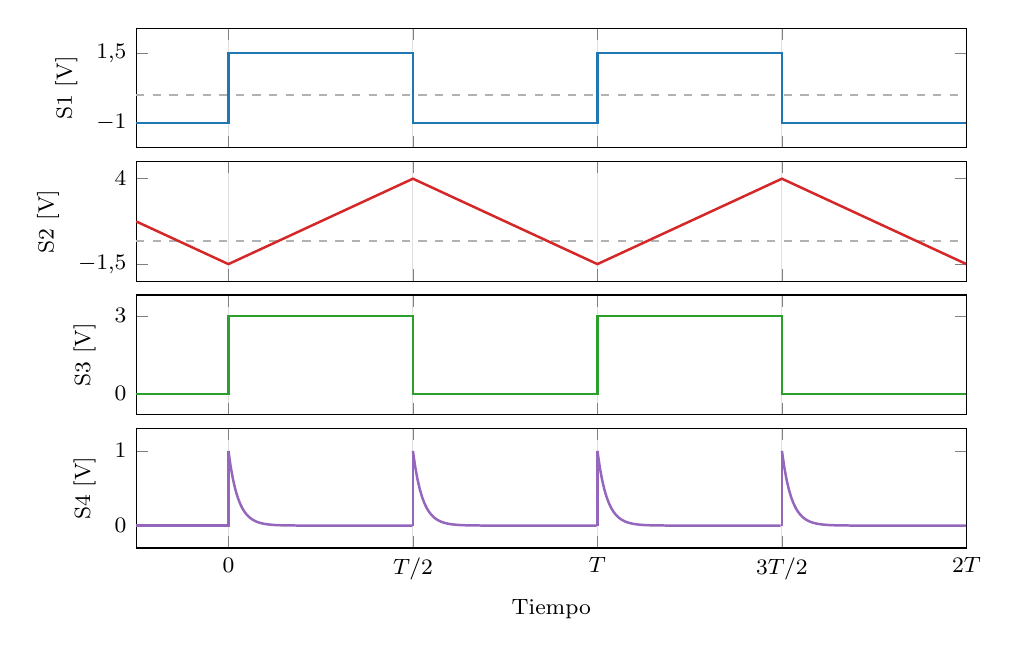
\begin{tikzpicture}
\begin{groupplot}[
    group style={group size=1 by 4, vertical sep=5pt, xticklabels at=edge bottom},
    tp2, height=3.1cm, xmin=-58.14, xmax=465.1,
    xtick={0,116.28,232.56,348.84,465.1}, xticklabels={$0$,$T/2$,$T$,$3T/2$,$2T$},
    ylabel style={font=\footnotesize}, yticklabel style={font=\footnotesize},
    ymajorgrids=false, xmajorgrids=true,
]
\nextgroupplot[ymin=-1.9, ymax=2.4, ytick={-1,1.5}, yticklabels={$-1$,$1{,}5$}, ylabel={S1 [V]}]
\addplot[gray!60, dashed, line width=0.5pt] coordinates {(-58.14,0) (465.1,0)};
\addplot[cs1, const plot] coordinates {(-58.14,-1) (0,1.5) (116.28,-1) (232.56,1.5) (348.84,-1) (465.1,-1)};
\nextgroupplot[ymin=-2.6, ymax=5.1, ytick={-1.5,4}, yticklabels={$-1{,}5$,$4$}, ylabel={S2 [V]}]
\addplot[gray!60, dashed, line width=0.5pt] coordinates {(-58.14,0) (465.1,0)};
\addplot[cs2] coordinates {(-58.14,1.25) (0,-1.5) (116.28,4) (232.56,-1.5) (348.84,4) (465.1,-1.5)};
\nextgroupplot[ymin=-0.8, ymax=3.8, ytick={0,3}, ylabel={S3 [V]}]
\addplot[cs3, const plot] coordinates {(-58.14,0) (0,3) (116.28,0) (232.56,3) (348.84,0) (465.1,0)};
\nextgroupplot[ymin=-0.3, ymax=1.3, ytick={0,1}, ylabel={S4 [V]}, xlabel={Tiempo}]
\addplot[cs4, domain=0:116, samples=80] {exp(-x/6)};
\addplot[cs4, domain=116.28:232, samples=80] {exp(-(x-116.28)/6)};
\addplot[cs4, domain=232.56:348, samples=80] {exp(-(x-232.56)/6)};
\addplot[cs4, domain=348.84:465, samples=80] {exp(-(x-348.84)/6)};
\addplot[cs4] coordinates {(-58.14,0) (0,0) (0,1)};
\addplot[cs4] coordinates {(116.28,0) (116.28,1)};
\addplot[cs4] coordinates {(232.56,0) (232.56,1)};
\addplot[cs4] coordinates {(348.84,0) (348.84,1)};
\end{groupplot}
\end{tikzpicture}
\caption{Señales pedidas por la consigna ($T = 1/\SI{4300}{\hertz} = \SI{232,6}{\micro\second}$). La línea de trazos marca \SI{0}{\volt}. La señal 2 sube mientras la señal 1 está en alto, la señal 3 está en alto mientras la señal 2 sube y la señal 4 tiene un impulso positivo de \SI{1}{\volt} en cada flanco de la señal 3.}
\label{fig:consigna}
\end{figure}

\subsection{Interpretación de las señales}
De la Fig.~\ref{fig:consigna} se leen las relaciones que debe cumplir cada etapa:
\begin{itemize}[leftmargin=*, nosep]
    \item \textbf{Señal 1}: cuadrada de \SI{-1}{\volt} a \SI{1,5}{\volt} (\SI{2,5}{\volt} pico a pico, valor medio \SI{0,25}{\volt}). El generador entrega una cuadrada de \SI{0}{} a \SI{2,5}{\volt}, de modo que la primera etapa le resta \SI{1}{\volt}.
    \item \textbf{Señal 2}: triangular de \SI{-1,5}{\volt} a \SI{4}{\volt} (\SI{5,5}{\volt} pico a pico, valor medio \SI{1,25}{\volt}). Es la integral de la señal 1 sin su valor medio y sin inversión: sube mientras la señal 1 está en alto. Su nivel de continua es el que la consigna pide fijar con la referencia de precisión.
    \item \textbf{Señal 3}: cuadrada de \SI{0}{} a \SI{3}{\volt}, en alto mientras la señal 2 sube. Sus flancos coinciden con los vértices de la triangular: la señal 3 indica el signo de la pendiente de la señal 2, es decir, es su derivada, desplazada y escalada.
    \item \textbf{Señal 4}: un impulso positivo de \SI{1}{\volt} que decae exponencialmente en cada flanco de la señal 3, tanto de subida como de bajada. Se obtiene derivando la señal 3, lo que da impulsos de signo alternado, y tomando su valor absoluto.
\end{itemize}

\subsection{Organización del informe}
La Sección~\ref{sec:diseno} desarrolla el diseño y su verificación por simulación. Para cada decisión explica qué alternativas había, por qué se eligió una, cómo se calcularon sus componentes y qué muestra la simulación. Incluye las hojas de datos y su análisis, el circuito completo y la impedancia de salida. La Sección~\ref{sec:impl} describe la implementación: la placa, el procedimiento de ajuste y medición y los resultados de las etapas que funcionaron como se esperaba. La Sección~\ref{sec:problemas} analiza lo que salió mal, en la medición y en las últimas etapas, y usa la simulación para acotar sus causas. La Sección~\ref{sec:conclusiones} reúne las conclusiones.

\section{Diseño y simulación}
\label{sec:diseno}

\subsection{Cómo se verificó cada decisión}
\label{sec:metodo}
Cada etapa se diseñó con las ecuaciones del operacional ideal y después se verificó con ngspice~\cite{ngspice}, usando modelos de los fabricantes, porque varios de los problemas de este circuito (la estabilidad del derivador, la conmutación del rectificador, la impedancia de salida) dependen justamente de lo que el modelo ideal no tiene. Se usaron los siguientes modelos:
\begin{itemize}[leftmargin=*, nosep]
    \item \textbf{TL084}: macromodelo de Texas Instruments, con entrada JFET, $B_1 = \SI{3}{\mega\hertz}$, $SR = \SI{13}{\volt\per\micro\second}$ y límites de excursión y de corriente de salida.
    \item \textbf{1N750}: modelo de onsemi, con ruptura a \SI{4,7}{\volt}.
    \item \textbf{1N4004}: parámetros de juntura de la familia 1N400x (Diodes Inc.), con tiempo de tránsito de \SI{5}{\micro\second}.
    \item \textbf{1N4148}: modelo de onsemi, con tiempo de tránsito de \SI{20}{\nano\second}, para comparar.
\end{itemize}
Cada análisis se hizo sobre el circuito completo de la Fig.~\ref{fig:circuito} o sobre la etapa en estudio, y todos los valores numéricos y las curvas de simulación de este informe salen directamente de esas corridas. Los presets se representan como dos resistores que suman \SI{10}{\kilo\ohm}; $P_1$ y $P_2$ se ajustan para $\Vrefd = \SI{1,25}{\volt}$ y $\Vrefu = \SI{1}{\volt}$ con la tensión del zener simulada (\valu{3}{\simVz}{\volt}), y $P_3$ para que el pico de la señal 4 sea de \SI{1}{\volt} (queda en \valu{2}{\simPtres}{\kilo\ohm}). Por el acoplamiento del integrador, el nivel medio de la triangular tarda decenas de milisegundos en establecerse; para no simular ese arranque en cada corrida, los capacitores $C_C$ y $C_1$ parten de sus tensiones de régimen, se simulan \SI{60}{\milli\second} con paso máximo de \SI{0,1}{\micro\second} y se analizan los últimos períodos.

\subsection{Elección del amplificador operacional}
\label{sec:opamp}
El circuito necesita once amplificadores, y antes de elegir el integrado conviene ver qué le exige cada etapa:
\begin{itemize}[leftmargin=*, nosep]
    \item \textbf{Corriente de polarización baja}. El integrador necesita una resistencia de \SI{1}{\mega\ohm} en la realimentación (Sección~\ref{sec:integrador}), y la corriente de polarización la recorre: \SI{80}{\nano\ampere} producirían \SI{80}{\milli\volt} de error en el nivel de la triangular.
    \item \textbf{\emph{Slew rate} alto}. Cada vez que un impulso de la señal 4 cambia de signo, el operacional del rectificador tiene que mover su salida unos \SI{2,5}{\volt} para pasar de un diodo al otro. Los impulsos duran unos \SI{5}{\micro\second}, así que ese salto tiene que durar una fracción de microsegundo.
    \item \textbf{Producto ganancia-ancho de banda alto}. Fija la frecuencia a la que tiende a oscilar el derivador y la impedancia de salida (Secciones~\ref{sec:derivador} y~\ref{sec:zout}).
    \item \textbf{Cuatro amplificadores por encapsulado}, para que once amplificadores entren en tres integrados.
\end{itemize}
La Tabla~\ref{tab:opamps} compara el TL084 con los operacionales de uso general que hay en el laboratorio. El LM741 y el LM324 tienen un \emph{slew rate} de \SI{0,5}{\volt\per\micro\second}: tardarían \SI{5}{\micro\second} en el salto del rectificador, tanto como dura el impulso, y lo deformarían por completo. Su corriente de polarización, de decenas de nanoampere, daría además decenas de milivolt de error en el integrador. El OP07 tiene un \emph{offset} cincuenta veces menor que el TL084, pero es todavía más lento y es simple: harían falta once integrados. El TL084 cumple las cuatro condiciones: su entrada JFET tiene una corriente de polarización mil veces menor que la de los bipolares, es veintiséis veces más rápido que el LM741 y es cuádruple. Su punto débil es el \emph{offset} de entrada, de hasta \SI{15}{\milli\volt}, y por eso el diseño evita amplificar la continua y deja ajustables los niveles. El TL082 es el mismo integrado en versión doble (haría falta el doble de integrados) y el TL074 es la versión de bajo ruido, que acá no aporta nada.

\begin{table}[!htb]
\centering
\caption{Operacionales de uso general (valores típicos de las hojas de datos~\cite{tl08x, opamps}).}
\label{tab:opamps}
\footnotesize
\setlength{\tabcolsep}{3.5pt}
\begin{tabular}{@{}lcccc@{}}
\toprule
 & \textbf{TL084} & \textbf{LM741} & \textbf{LM324} & \textbf{OP07} \\
\midrule
Entrada & JFET & bipolar & bipolar & bipolar \\
\emph{Slew rate} [\si{\volt\per\micro\second}] & 13 & 0,5 & 0,5 & 0,3 \\
Ganancia-ancho de banda [\si{\mega\hertz}] & 3 & 1 & 1 & 0,6 \\
Corriente de polarización [\si{\nano\ampere}] & 0,03 & 80 & 20 & 1 \\
\emph{Offset} de entrada [\si{\milli\volt}] & 3 & 1 & 2 & 0,06 \\
Amplificadores por integrado & 4 & 1 & 4 & 1 \\
Integrados para este circuito & 3 & 11 & 3 & 11 \\
\bottomrule
\end{tabular}
\end{table}

De la hoja de datos del TL084C~\cite{tl08x} interesan además los parámetros que la consigna pide analizar y que no aparecen en la Tabla~\ref{tab:opamps}. El rechazo de modo común es de \SI{86}{\deci\bel} típico (\SI{70}{\deci\bel} mínimo): en el restador de la señal 1 el modo común no pasa de \SI{1,25}{\volt}, lo que da un error de \SI{0,4}{\milli\volt}, despreciable frente al que introduce el apareamiento de los resistores (Sección~\ref{sec:s1}). El tiempo de crecimiento en pequeña señal es de \SI{0,05}{\micro\second}, y en gran señal manda el \emph{slew rate}: \SI{13}{\volt\per\micro\second} típico y \SI{8}{\volt\per\micro\second} mínimo, con lo que el flanco de \SI{2,5}{\volt} de la señal 1 dura \SI{0,2}{\micro\second}, el \SI{0,08}{\percent} del período. El \emph{offset} de entrada es de \SI{3}{\milli\volt} típico y \SI{15}{\milli\volt} máximo, con una deriva de \SI{18}{\micro\volt\per\celsius}; la corriente de polarización, de \SI{30}{\pico\ampere} típica y \SI{400}{\pico\ampere} máxima, produce sobre $R_F = \SI{1}{\mega\ohm}$ menos de \SI{0,4}{\milli\volt}. Con $\pm\SI{12}{\volt}$ la salida llega a unos $\pm\SI{10,5}{\volt}$, más del doble de la mayor excursión del circuito.

\subsection{Alimentación}
\label{sec:alim}
Las señales van de \SI{-1,5}{} a \SI{4}{\volt}, así que el circuito necesita una fuente partida: con fuente simple habría que correr todos los niveles hacia arriba y volver a bajarlos al final. Se eligió $\pm\SI{12}{\volt}$ y no $\pm\SI{15}{\volt}$ porque alcanza con holgura: con \SI{12}{\volt} el TL084 llega a unos $\pm\SI{10,5}{\volt}$ de salida, más del doble de la mayor excursión del circuito, y su rango de modo común (unos \SI{9}{\volt} hacia el negativo) queda muy lejos de las señales. Además, con menos tensión cada integrado disipa menos y $R_Z$ también. Cada integrado tiene un capacitor cerámico de \SI{100}{\nano\farad} entre cada pin de alimentación y masa, lo más cerca posible del integrado, que entrega la corriente de los transitorios rápidos, y uno electrolítico de \SI{10}{\micro\farad} que cubre las variaciones lentas de consumo.

\subsection{Arquitectura y ganancia de cada etapa}
\label{sec:arq}
La Fig.~\ref{fig:bloques} muestra la cadena de etapas y la Fig.~\ref{fig:circuito}, el circuito completo. La organización sigue tres criterios.

\textbf{Cada señal sale de un operacional realimentado}, con impedancia de salida baja, para que la etapa siguiente no la cargue ni cambie su forma.

\textbf{Los niveles de continua vienen de una referencia}, no de divisores sobre la fuente de \SI{12}{\volt}: un divisor transmite a la señal cualquier variación de la fuente en la misma proporción, mientras que con el zener la variación relativa es unas diez veces menor (Sección~\ref{sec:ref}).

\textbf{Se amplifica donde la señal se genera, y la continua nunca con ganancia mayor que 2.} El \emph{offset} del TL084 llega a \SI{15}{\milli\volt}: una etapa que amplificara la continua por 4, por ejemplo, convertiría eso en \SI{60}{\milli\volt} de error de nivel. Por eso el integrador se dimensiona para dar directamente los \SI{5,5}{\volt} de la triangular, en vez de integrar una señal chica y amplificarla después, y el derivador da directamente los $\pm\SI{1,5}{\volt}$ de la señal 3. La Tabla~\ref{tab:ganancias} resume la ganancia de cada etapa y por qué.

\begin{figure}[!htb]
\centering
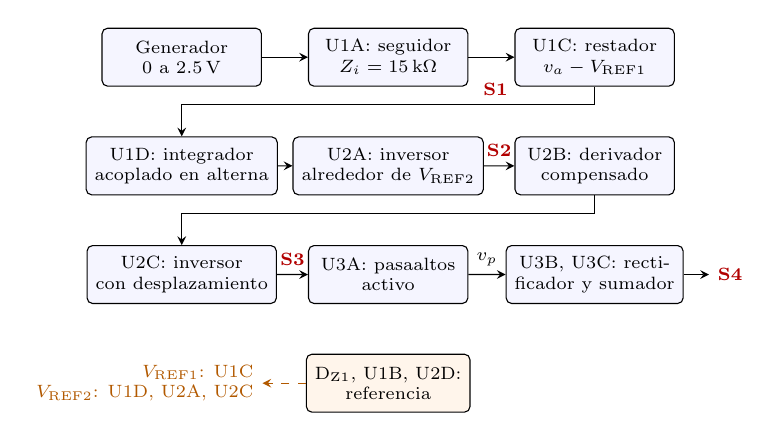
\begin{tikzpicture}[scale=0.92, transform shape, font=\scriptsize,
    b/.style={draw, rounded corners=2pt, minimum width=2.2cm, minimum height=0.8cm, align=center, fill=blue!4},
    r/.style={draw, rounded corners=2pt, minimum width=2.2cm, minimum height=0.8cm, align=center, fill=orange!8},
    s/.style={font=\scriptsize\bfseries, color=red!70!black},
    ->, >=stealth]
\node[b] (gen) at (0,0) {Generador\\0 a \SI{2,5}{\volt}};
\node[b] (u1a) at (2.85,0) {U1A: seguidor\\$Z_i = \SI{15}{\kilo\ohm}$};
\node[b] (u1c) at (5.7,0) {U1C: restador\\$v_a - \Vrefu$};
\node[b] (u1d) at (0,-1.5) {U1D: integrador\\acoplado en alterna};
\node[b] (u2a) at (2.85,-1.5) {U2A: inversor\\alrededor de $\Vrefd$};
\node[b] (u2b) at (5.7,-1.5) {U2B: derivador\\compensado};
\node[b] (u2c) at (0,-3.0) {U2C: inversor\\con desplazamiento};
\node[b] (u3a) at (2.85,-3.0) {U3A: pasaaltos\\activo};
\node[b] (u3b) at (5.7,-3.0) {U3B, U3C: recti-\\ficador y sumador};
\node[r] (ref) at (2.85,-4.5) {D\textsubscript{Z1}, U1B, U2D:\\referencia};
\draw (gen) -- (u1a);
\draw (u1a) -- (u1c);
\draw (u1c.south) -- ++(0,-0.25) -| node[s, pos=0.12, above] {S1} (u1d.north);
\draw (u1d) -- (u2a);
\draw (u2a) -- node[s, above] {S2} (u2b);
\draw (u2b.south) -- ++(0,-0.25) -| (u2c.north);
\draw (u2c) -- node[s, above] {S3} (u3a);
\draw (u3a) -- node[above] {$v_p$} (u3b);
\draw (u3b.east) -- ++(0.35,0) node[s, right] {S4};
\draw[dashed, color=orange!70!black] (ref.west) -- ++(-0.6,0) node[left, align=right] {$\Vrefu$: U1C\\$\Vrefd$: U1D, U2A, U2C};
\end{tikzpicture}
\caption{Cadena de etapas. Cada bloque es un amplificador de los tres TL084; la referencia alimenta a los bloques que fijan niveles.}
\label{fig:bloques}
\end{figure}

\begin{table}[!htb]
\centering
\caption{Ganancia de cada etapa y su justificación.}
\label{tab:ganancias}
\footnotesize
\setlength{\tabcolsep}{3pt}
\begin{tabular}{@{}l>{\centering}p{1.3cm}>{\raggedright\arraybackslash}p{4.6cm}@{}}
\toprule
\textbf{Etapa} & \textbf{Ganancia} & \textbf{Por qué} \\
\midrule
U1A & $1$ & El generador ya entrega los \SI{2,5}{\volt} pico a pico de la señal 1; solo hay que fijar $Z_i$. \\
U1C & $1$ & La señal 1 tiene la misma amplitud que la entrada; solo cambia el nivel. \\
U1D & $1/(sR_IC_1)$ & Da directamente los \SI{5,5}{\volt} de la triangular: no hace falta amplificarla después. \\
U2A & $-1$ & Corrige el signo y pone el nivel en $\Vrefd$; la amplitud ya es la correcta. \\
U2B & $-sR_DC_D$ & Da directamente los $\pm\SI{1,5}{\volt}$ que necesita la señal 3. \\
U2C & $-1$ & Corrige el signo y suma \SI{1,5}{\volt}. \\
U3A & $-1$ (alta frec.) & Genera los impulsos sin cambiar su escala. \\
U3B, U3C & $0{,}5$ a $1$ & Rectifica y ajusta con $P_3$ el pico final de \SI{1}{\volt}, igual para los dos flancos. \\
\bottomrule
\end{tabular}
\end{table}

\begin{figure*}[!t]
\centering
% Circuito completo del TP2 (3 x TL084, alimentacion +/-12 V).
% Se incluye con \input dentro de un figure*. Coordenadas absolutas.
\begin{circuitikz}[scale=0.62, transform shape, font=\small]
\ctikzset{resistors/scale=0.7, capacitors/scale=0.7, diodes/scale=0.7,
          tripoles/op amp/width=1.5, tripoles/op amp/height=1.5,
          tripoles/op amp/input height=0.5, bipoles/length=1.2cm}
\tikzset{et/.style={font=\footnotesize\bfseries, color=blue!55!black},
         senal/.style={font=\normalsize\bfseries, color=red!70!black},
         ref/.style={font=\small}}

% =============================== FILA 1 ===============================
% ---- Entrada y adaptacion de impedancia (U1A) ----
\node[et, align=center] at (2.4,3.3) {Adaptación de $Z_i$};
\draw (0,0) node[ocirc] {} node[above, align=center, font=\footnotesize, yshift=2pt]
      {Generador\\0 a \SI{2,5}{\volt}\\\SI{4300}{\hertz}};
\draw (0.08,0) to[short, -*] (0.9,0) to[R, l_={$R_1$\\\SI{15}{\kilo\ohm}}, align=left] (0.9,-1.8) node[ground] {};
\node[op amp, noinv input up, anchor=+] (u1a) at (2.0,0) {\scriptsize U1A};
\draw (0.9,0) -- (u1a.+);
\draw (u1a.-) -- (1.7,-1.0) -- (1.7,-1.7) -- (4.4,-1.7) -- (4.4,-0.5);
\draw (u1a.out) to[short, -*] (4.4,-0.5);

% ---- Senal 1: amplificador diferencial (U1C) ----
\node[et] at (8.0,3.3) {Señal 1};
\draw (4.4,-0.5) to[R, l={$R_2$ \SI{10}{\kilo\ohm}}] (6.4,-0.5) to[short, -*] (6.7,-0.5);
\node[op amp, anchor=-] (u1c) at (7.2,0.5) {\scriptsize U1C};
\draw (6.7,-0.5) -- (u1c.+);
\draw (6.7,-0.5) to[R, l_={$R_3$\\\SI{10}{\kilo\ohm}}, align=right] (6.7,-2.3) node[ground] {};
\draw (u1c.-) to[short, -*] (6.9,0.5);
\draw (6.9,0.5) to[R, l_={$R_4$ \SI{10}{\kilo\ohm}}] (5.0,0.5) node[left, ref] {$V_{\mathrm{REF1}}$};
\draw (6.9,0.5) -- (6.9,1.6) to[R, l={$R_5$ \SI{10}{\kilo\ohm}}] (9.6,1.6) -- (9.6,0) -- (u1c.out);
\draw (9.6,0) to[short, *-*] (10.0,0);
\node[senal, below] at (10.0,-0.1) {S1};

% ---- Integrador con acoplamiento capacitivo (U1D) ----
\node[et] at (14.6,3.3) {Integrador};
\draw (10.0,0) to[C, l={$C_C$ \SI{1}{\micro\farad}}] (11.7,0)
      to[R, l={$R_I$ \SI{5,6}{\kilo\ohm}}] (13.4,0) to[short, -*] (13.7,0);
\node[op amp, anchor=-] (u1d) at (14.2,0) {\scriptsize U1D};
\draw (13.7,0) -- (u1d.-);
\draw (13.7,0) -- (13.7,1.1) to[C, l={$C_1$ \SI{4,7}{\nano\farad}}] (16.6,1.1);
\draw (13.7,1.1) to[short, *-] (13.7,2.2) to[R, l={$R_F$ \SI{1}{\mega\ohm}}] (16.6,2.2) -- (16.6,1.1) to[short, *-] (16.6,-0.5) -- (u1d.out);
\draw (u1d.+) -- (13.9,-1.0) node[left, ref] {$V_{\mathrm{REF2}}$};
\draw (16.6,-0.5) to[short, *-] (16.9,-0.5);

% ---- Senal 2: inversor alrededor de VREF2 (U2A) ----
\node[et] at (20.6,3.3) {Señal 2};
\draw (16.9,-0.5) to[R, l={$R_6$ \SI{10}{\kilo\ohm}}] (18.7,-0.5) to[short, -*] (19.0,-0.5);
\node[op amp, anchor=-] (u2a) at (19.5,-0.5) {\scriptsize U2A};
\draw (19.0,-0.5) -- (u2a.-);
\draw (19.0,-0.5) -- (19.0,0.6) to[R, l={$R_7$ \SI{10}{\kilo\ohm}}] (21.9,0.6) -- (21.9,-1.0) -- (u2a.out);
\draw (u2a.+) -- (19.2,-1.5) node[left, ref] {$V_{\mathrm{REF2}}$};
\draw (21.9,-1.0) to[short, *-*] (22.4,-1.0);
\node[senal, right] at (22.5,-1.0) {S2};

% =============================== FILA 2 ===============================
% ---- Referencia de precision con buffer (DZ1, P1, P2, U1B, U2D) ----
\node[et, align=center] at (3.0,-3.0) {Referencia de precisión};
\draw (0.6,-3.7) node[vcc] {$+\SI{12}{\volt}$} to[R, l_={$R_Z$\\\SI{470}{\ohm}}, align=left] (0.6,-5.2);
\draw (0.6,-7.0) node[ground] {} to[zDo, l^={$D_{Z1}$\\1N750\\\SI{4,7}{\volt}}, align=right, -*] (0.6,-5.2);
\draw (0.6,-5.2) to[short, -*] (1.3,-5.2) -- (1.9,-5.2) to[pR, n=pa, l_={$P_1$}, mirror] (1.9,-7.0) node[ground] {};
\draw (1.3,-5.2) -- (1.3,-8.3) -- (1.9,-8.3) to[pR, n=pb, l_={$P_2$}, mirror] (1.9,-10.1) node[ground] {};
\node[op amp, noinv input up, anchor=+] (u1b) at (3.0,-6.1) {\scriptsize U1B};
\draw (pa.wiper) -| (2.7,-6.1) -- (u1b.+);
\draw (u1b.-) -- (2.75,-7.1) -- (2.75,-7.6) -- (5.4,-7.6) -- (5.4,-6.6) -- (u1b.out);
\draw (5.4,-6.6) to[short, *-o] (5.8,-6.6) node[right, ref] {$V_{\mathrm{REF2}}$};
\node[op amp, noinv input up, anchor=+] (u2d) at (3.0,-9.2) {\scriptsize U2D};
\draw (pb.wiper) -| (2.7,-9.2) -- (u2d.+);
\draw (u2d.-) -- (2.75,-10.2) -- (2.75,-10.7) -- (5.4,-10.7) -- (5.4,-9.7) -- (u2d.out);
\draw (5.4,-9.7) to[short, *-o] (5.8,-9.7) node[right, ref] {$V_{\mathrm{REF1}}$};
\node[font=\footnotesize, align=left, anchor=west] at (0.0,-11.6)
     {$P_1$, $P_2$: preset multivuelta \SI{10}{\kilo\ohm}\\
      $V_{\mathrm{REF2}} = \SI{1,25}{\volt}$, $V_{\mathrm{REF1}} = \SI{1,00}{\volt}$};

% ---- Derivador compensado (U2B) ----
\node[et] at (10.3,-3.5) {Derivador};
\draw (22.4,-1.0) -- (22.4,-2.8) -- (9.0,-2.8) -- (9.0,-5.8);
\draw (9.0,-5.8) to[R, l_={$R_S$ \SI{1}{\kilo\ohm}}] (10.6,-5.8)
      to[C, l_={$C_D$ \SI{1}{\nano\farad}}] (12.2,-5.8) to[short, -*] (12.5,-5.8);
\node[op amp, anchor=-] (u2b) at (13.0,-5.8) {\scriptsize U2B};
\draw (12.5,-5.8) -- (u2b.-);
\draw (u2b.+) -- (12.7,-6.8) node[ground] {};
\draw (12.5,-5.8) -- (12.5,-4.8) to[C, l={$C_F$ \SI{56}{\pico\farad}}] (15.4,-4.8);
\draw (12.5,-4.8) to[short, *-] (12.5,-3.8) to[R, l={$R_D$ \SI{31,6}{\kilo\ohm}}] (15.4,-3.8) -- (15.4,-4.8) to[short, *-] (15.4,-6.3) -- (u2b.out);
\draw (15.4,-6.3) to[short, *-] (15.7,-6.3);

% ---- Senal 3: inversor con desplazamiento (U2C) ----
\node[et] at (19.4,-3.5) {Señal 3};
\draw (15.7,-6.3) to[R, l={$R_{10}$ \SI{10}{\kilo\ohm}}] (17.5,-6.3) to[short, -*] (17.8,-6.3);
\node[op amp, anchor=-] (u2c) at (18.3,-6.3) {\scriptsize U2C};
\draw (17.8,-6.3) -- (u2c.-);
\draw (17.8,-6.3) -- (17.8,-5.2) to[R, l={$R_{11}$ \SI{10}{\kilo\ohm}}] (20.7,-5.2) -- (20.7,-6.8) -- (u2c.out);
\draw (u2c.+) to[short, -*] (17.9,-7.3);
\draw (17.9,-7.3) to[R, l_={$R_9$\\\SI{15}{\kilo\ohm}}, align=right] (17.9,-9.0) node[ground] {};
\draw (17.9,-7.3) to[R, l_={$R_8$ \SI{10}{\kilo\ohm}}] (16.0,-7.3) node[left, ref] {$V_{\mathrm{REF2}}$};
\draw (20.7,-6.8) to[short, *-*] (21.1,-6.8);
\node[senal, right] at (21.2,-6.8) {S3};

% =============================== FILA 3 ===============================
% ---- Generador de impulsos: pasaaltos activo (U3A) ----
\node[et, align=center] at (13.6,-14.9) {Generador de impulsos};
\draw (21.1,-6.8) -- (21.1,-9.8) -- (8.6,-9.8) -- (8.6,-12.5);
\draw (8.6,-12.5) to[R, l_={$R_{S4}$ \SI{4,7}{\kilo\ohm}}] (10.3,-12.5)
      to[C, l_={$C_4$ \SI{1}{\nano\farad}}] (11.9,-12.5) to[short, -*] (12.2,-12.5);
\node[op amp, anchor=-] (u3a) at (12.7,-12.5) {\scriptsize U3A};
\draw (12.2,-12.5) -- (u3a.-);
\draw (u3a.+) -- (12.4,-13.5) node[ground] {};
\draw (12.2,-12.5) -- (12.2,-11.4) to[R, l={$R_{F4}$ \SI{4,7}{\kilo\ohm}}] (15.1,-11.4) -- (15.1,-13.0) -- (u3a.out);
\draw (15.1,-13.0) to[short, *-*] (15.5,-13.0);
\node[font=\small, below left] at (15.5,-13.0) {$v_p$};

% ---- Rectificador de precision (U3B) ----
\node[et, align=center] at (19.4,-16.4) {Rectificador de precisión};
\draw (15.5,-13.0) to[R, l_={$R_{12}$ \SI{10}{\kilo\ohm}}] (17.3,-13.0) to[short, -*] (17.6,-13.0);
\node[op amp, anchor=-] (u3b) at (18.2,-13.0) {\scriptsize U3B};
\draw (17.6,-13.0) -- (u3b.-);
\draw (u3b.+) node[ground] {};
\draw (u3b.out) to[short, -*] (20.6,-13.5);
\draw (20.6,-13.5) -- (20.6,-11.8) to[D, l^={$D_1$ 1N4004}] (17.6,-11.8) -- (17.6,-13.0);
\draw (17.6,-13.0) -- (17.6,-15.2) to[R, l_={$R_{13}$ \SI{10}{\kilo\ohm}}] (21.4,-15.2);
\draw (21.4,-15.2) to[D, l_={$D_2$\\1N4004}, align=left, *-] (21.4,-13.5) -- (20.6,-13.5);
\node[font=\small, below left] at (21.4,-15.2) {$v_A$};

% ---- Sumador de salida (U3C): senal 4 ----
\node[et] at (25.9,-10.9) {Sumador};
\draw (15.5,-13.0) -- (15.5,-10.4) to[R, l_={$R_{14}$ \SI{20}{\kilo\ohm}}] (23.4,-10.4) -- (23.4,-13.0);
\draw (21.4,-15.2) to[R, l_={$R_{15}$ \SI{10}{\kilo\ohm}}] (23.4,-15.2) -- (23.4,-13.0);
\node[op amp, noinv input up, anchor=-] (u3c) at (24.2,-13.0) {\scriptsize U3C};
\draw (23.4,-13.0) to[short, *-*] (23.8,-13.0) -- (u3c.-);
\draw (u3c.+) -- (23.9,-12.0) node[ground] {};
\draw (23.8,-13.0) -- (23.8,-16.4) to[R, l_={$R_{F8}$ \SI{10}{\kilo\ohm}}] (25.3,-16.4)
      to[vR, l_={$P_3$ \SI{10}{\kilo\ohm}}] (26.8,-16.4) -- (26.8,-12.5) -- (u3c.out);
\draw (26.8,-12.5) to[short, *-o] (27.3,-12.5);
\node[senal, right] at (27.4,-12.5) {S4};

% ---- Notas ----
\node[font=\footnotesize, align=left, anchor=north west] at (0.0,-13.2)
     {U1, U2, U3: TL084 (U3D sin uso).\\
      Alimentación: $\pm\SI{12}{\volt}$, desacople de\\
      \SI{100}{\nano\farad} + \SI{10}{\micro\farad} en cada integrado.\\
      Resistores de película metálica, \SI{1}{\percent}.};
\end{circuitikz}

\caption{Circuito completo. S1 a S4 son las cuatro señales de la consigna. Los nodos marcados $\Vrefu$ y $\Vrefd$ se conectan a las salidas de U2D y U1B. El cuarto amplificador de U3 queda sin uso, conectado como seguidor con la entrada a masa.}
\label{fig:circuito}
\end{figure*}

El período de la señal es $T = 1/\SI{4300}{\hertz} = \SI{232,56}{\micro\second}$ y cada semiperíodo dura $T/2 = \SI{116,28}{\micro\second}$. Salvo indicación, los resistores son de película metálica con tolerancia del \SI{1}{\percent}: los niveles de varias etapas dependen de cocientes entre resistores, y con resistores de carbón del \SI{5}{\percent} esos cocientes podrían errar un \SI{10}{\percent}.

\subsection{Entrada: impedancia de \SI{15}{\kilo\ohm} (U1A)}
\label{sec:entrada}
\paragraph*{Alternativas} La forma más directa de fijar una impedancia de entrada es la resistencia de entrada de un amplificador inversor: con \SI{15}{\kilo\ohm} en serie con la entrada inversora, $Z_i = \SI{15}{\kilo\ohm}$. Pero esa etapa invierte la señal y su ganancia queda atada a los \SI{15}{\kilo\ohm} ($-R_F/\SI{15}{\kilo\ohm}$). Se eligió terminar la entrada en $R_1 = \SI{15}{\kilo\ohm}$ a masa y tomarla con el seguidor U1A:
\begin{equation}
Z_i = R_1 \parallel r_i \approx \SI{15}{\kilo\ohm},
\end{equation}
porque la resistencia de entrada del TL084 es de $\SI{e12}{\ohm}$ y su capacidad de entrada, de pocos picofaradios. Así $Z_i$ depende de un solo resistor del \SI{1}{\percent} y no de lo que venga después, y la señal no se invierte.

\paragraph*{Por qué hace falta el seguidor} Sin U1A, el restador de la señal 1 quedaría en paralelo con $R_1$; su resistencia de entrada es de \SI{20}{\kilo\ohm} y bajaría la impedancia de entrada a \SI{8,6}{\kilo\ohm}. El seguidor tiene ganancia 1 porque no hay nada que amplificar: el generador ya entrega la amplitud de la señal 1. La simulación da $Z_i = \valu{2}{\simZin}{\kilo\ohm}$, constante hasta \SI{1}{\mega\hertz}.

\subsection{Referencia de precisión con buffer (D\textsubscript{Z1}, U1B, U2D)}
\label{sec:ref}
\paragraph*{Por qué un zener y no un divisor} Un divisor resistivo sobre la fuente de \SI{12}{\volt} transmite a la referencia cualquier variación de la fuente: un \SI{10}{\percent} menos de alimentación movería los niveles un \SI{10}{\percent}. El zener se polariza con $R_Z$ desde $+\SI{12}{\volt}$ y su tensión cambia solo en la proporción del divisor que forman $R_Z$ y su impedancia dinámica $Z_Z$:
\begin{equation}
\frac{\Delta \Vrefd}{\Delta V_{CC}} = \alpha_1 \frac{Z_Z}{R_Z + Z_Z},
\end{equation}
donde $\alpha_1$ es la fracción de $V_Z$ que toma el preset. Con el máximo de la hoja de datos, $Z_Z = \SI{19}{\ohm}$~\cite{1n750}, una variación de $\pm\SI{10}{\percent}$ en la fuente mueve $\Vrefd$ en $\pm\SI{12}{\milli\volt}$ ($\pm\SI{1}{\percent}$), diez veces menos que con un divisor. Con el modelo SPICE, cuya impedancia dinámica es de \valu{1}{\simZz}{\ohm}, la simulación da \valu{1}{\simRefLinea}{\milli\volt} entre \SI{10,8}{} y \SI{13,2}{\volt}. Una referencia integrada de banda prohibida (TL431, LM336) tendría mejor coeficiente de temperatura, pero los niveles de la consigna se leen con una resolución de décimas de volt y el zener con preset alcanza con margen. Es además el esquema de zener más amplificador que describe la nota de aplicación de la cátedra~\cite{refs}.

\paragraph*{Zener y $R_Z$} Se usa un 1N750, de \SI{4,7}{\volt} y \SI{500}{\milli\watt}~\cite{1n750}. Su tensión deja \SI{7,3}{\volt} sobre $R_Z$ para fijar la corriente, y las dos referencias necesarias (\SI{1}{} y \SI{1,25}{\volt}) son una fracción cómoda de ella. La tolerancia de $V_Z$ no importa porque las referencias se ajustan con presets. La impedancia dinámica de un zener baja con la corriente, así que conviene polarizarlo cerca de los \SI{20}{\milli\ampere} de su especificación, sin calentar $R_Z$. Con $R_Z = \SI{470}{\ohm}$ y $V_Z = \SI{4,69}{\volt}$,
\begin{equation}
I_{R_Z} = \frac{\SI{12}{\volt} - V_Z}{R_Z} = \SI{15,6}{\milli\ampere},
\end{equation}
de los que \SI{0,94}{\milli\ampere} van a los presets y \SI{14,6}{\milli\ampere} al zener. El zener disipa \SI{68}{\milli\watt} (\SI{14}{\percent} de su máximo) y $R_Z$, \SI{114}{\milli\watt}, dentro de lo admisible para un resistor de \SI{0,25}{\watt}. El modelo de onsemi tiene un coeficiente de temperatura de \SI{-21}{\ppm\per\celsius}: entre \SI{0}{} y \SI{40}{\celsius} la referencia de \SI{1,25}{\volt} cambia \SI{1,1}{\milli\volt}.

\paragraph*{Presets} Cada preset toma una fracción de $V_Z$: $\alpha_1 = \SI{1,25}{\volt}/V_Z = 0{,}267$ para $\Vrefd$ y $\alpha_2 = \SI{1}{\volt}/V_Z = 0{,}213$ para $\Vrefu$. Son multivuelta de \SI{10}{\kilo\ohm}: con 25 vueltas para \SI{4,7}{\volt}, cada vuelta mueve la referencia \SI{0,19}{\volt}, de modo que el ajuste fino llega al milivolt; y \SI{10}{\kilo\ohm} es lo bastante alto para tomar solo \SI{0,47}{\milli\ampere} del zener. Se usan dos referencias independientes porque la consigna fija dos niveles distintos (el de la señal 1 y el de la señal 2) y así cada uno se ajusta sin mover el otro.

\paragraph*{Por qué el buffer} El cursor de un preset de \SI{10}{\kilo\ohm} en esa posición tiene una resistencia de Thévenin de unos \SI{2}{\kilo\ohm}, comparable con las resistencias que alimenta: $\Vrefu$ entra por $R_4 = \SI{10}{\kilo\ohm}$ al restador, y $\Vrefd$ alimenta el divisor $R_8$--$R_9$ de \SI{25}{\kilo\ohm}. Sin seguidores, esa resistencia se sumaría a $R_4$ y desbalancearía el restador, y la corriente variable de cada etapa movería la referencia. Los seguidores U1B y U2D entregan las referencias con impedancia de salida de fracciones de ohm: esta es la ``referencia de precisión con un \emph{buffer}'' que pide la consigna.

\subsection{Señal 1: restador (U1C)}
\label{sec:s1}
\paragraph*{Alternativas} Para restar \SI{1}{\volt} hay dos opciones con un operacional: un sumador inversor, que daría $-(v_a - \SI{1}{\volt})$ y obligaría a agregar otro inversor, o un amplificador diferencial, que resta sin invertir. Se eligió el diferencial, con cuatro resistores iguales:
\begin{equation}
\sen{1} = \frac{R_3}{R_2 + R_3}\left(1 + \frac{R_5}{R_4}\right) v_a - \frac{R_5}{R_4}\,\Vrefu = v_a - \Vrefu,
\end{equation}
donde $v_a$ es la salida del seguidor de entrada. Con $v_a$ de \SI{0}{} a \SI{2,5}{\volt} y $\Vrefu = \SI{1}{\volt}$, $\sen{1}$ va de \SI{-1}{} a \SI{1,5}{\volt}. La ganancia es 1 porque la señal 1 tiene la misma amplitud que la entrada.

\paragraph*{Valores} \SI{10}{\kilo\ohm} es lo bastante alto para que U1A y U2D entreguen como máximo \SI{0,25}{\milli\ampere}, y lo bastante bajo para que las capacidades parásitas de pocos picofaradios formen polos por encima de los megahertz. La ganancia para $v_a$ es exactamente 1 solo si $R_3/R_2 = R_5/R_4$, y por eso los resistores son del \SI{1}{\percent}: el error de ganancia queda por debajo del \SI{2}{\percent} (\SI{50}{\milli\volt} sobre \SI{2,5}{\volt}). El nivel se corrige con $P_2$, que también compensa el \emph{offset} de U1C (ganancia de ruido 2, hasta \SI{30}{\milli\volt}).

\subsection{Señal 2: integrador (U1D) e inversor (U2A)}
\label{sec:integrador}
\paragraph*{Topología} La triangular es la integral de la cuadrada. Se usa el integrador inversor (de Miller), que tiene una sola constante de tiempo y no depende del apareamiento de resistores, a diferencia del integrador no inversor de Deboo. Su inversión se corrige con U2A, que hace falta de todos modos para fijar el nivel de la señal 2.

\paragraph*{Pendiente y amplitud} La señal 1 vale $\langle \sen{1} \rangle + \SI{1,25}{\volt}$ en el semiperíodo alto y $\langle \sen{1} \rangle - \SI{1,25}{\volt}$ en el bajo. El integrador la convierte en rampas de pendiente $\pm\SI{1,25}{\volt}/(R_I C_1)$, y para que la triangular tenga \SI{5,5}{\volt} pico a pico hace falta
\begin{equation}
R_I C_1 = \frac{\SI{1,25}{\volt} \cdot T/2}{\SI{5,5}{\volt}} = \SI{26,4}{\micro\second}.
\label{eq:ric1}
\end{equation}
Se eligió $C_1 = \SI{4,7}{\nano\farad}$ y $R_I = \SI{5,6}{\kilo\ohm}$ ($R_I C_1 = \SI{26,3}{\micro\second}$: \SI{5,52}{\volt} pico a pico y \SI{47,5}{\volt\per\milli\second}). Con un capacitor diez veces mayor, $R_I$ sería de \SI{560}{\ohm} y U1C tendría que entregar \SI{2,2}{\milli\ampere}; con uno diez veces menor, las capacidades parásitas de la placa serían una fracción apreciable de $C_1$. $C_1$ es de poliéster del \SI{5}{\percent}, porque la amplitud de la triangular depende directamente de su valor y un cerámico de uso general cambia hasta un \SI{20}{\percent} con la temperatura y con la tensión aplicada.

\paragraph*{El problema de la continua} Un integrador ideal tiene ganancia infinita en continua: el valor medio de la señal 1 (\SI{0,25}{\volt}) y el \emph{offset} del operacional lo saturan en pocos milisegundos. La solución habitual es una resistencia $R_F$ en paralelo con $C_1$~\cite{linares-intder}, que limita la ganancia en continua a $-R_F/R_I$, pero eso obliga a un compromiso:
\begin{itemize}[leftmargin=*, nosep]
    \item Cada rampa es en realidad una exponencial de constante $R_F C_1$, y su pendiente al final del semiperíodo es $e^{-T/(2 R_F C_1)}$ veces la del principio. Con $R_F/R_I = 10$ ese factor es 0,64.
    \item Si se aumenta $R_F$ para mejorar la linealidad, también crece la ganancia en continua, y cualquier error $\varepsilon$ en el valor medio de la entrada desplaza la triangular $(R_F/R_I)\,\varepsilon$. Con $R_F/R_I = 100$ las rampas son casi rectas, pero \SI{50}{\milli\volt} de error mueven el nivel \SI{5}{\volt}.
\end{itemize}
Por eso se agrega $C_C$ en serie con $R_I$. Para la continua la entrada queda abierta: el valor medio de la señal 1 no llega al integrador, $C_C$ se carga con $\langle \sen{1} \rangle - \Vrefd = \SI{-1}{\volt}$ y la única realimentación en continua es $R_F$, con ganancia de ruido 1. La salida queda centrada en el potencial de la entrada no inversora, $\Vrefd$, con un error igual al \emph{offset} de U1D. La transferencia completa es
\begin{equation}
\frac{V_{int}}{V_{S1}}(s) = -\frac{s C_C R_F}{(1 + s R_I C_C)(1 + s R_F C_1)},
\end{equation}
que por encima de los polos en $1/(2\pi R_I C_C) = \SI{28}{\hertz}$ y $1/(2\pi R_F C_1) = \SI{34}{\hertz}$ se reduce a $-1/(s R_I C_1)$.

\paragraph*{$C_C$ y $R_F$} Con $C_C$ acoplando la entrada, $R_F$ ya no fija el nivel y puede ser grande. Con \SI{1}{\mega\ohm} se pierden por ella como máximo \SI{2,8}{\micro\ampere}, contra \SI{223}{\micro\ampere} de corriente de integración; con un valor mayor, la corriente de polarización empezaría a pesar y el arranque sería aún más lento. $C_C = \SI{1}{\micro\farad}$ hace que $R_I C_C = \SI{5,6}{\milli\second}$, cincuenta veces el semiperíodo, de modo que la corriente por $R_I$ decae solo un \SI{2}{\percent} durante cada rampa. $C_C$ es de poliéster y no electrolítico: la corriente de fuga de un electrolítico, del orden del microampere, entraría al nodo de integración y saldría por $R_F$, y \SI{1}{\micro\ampere} por \SI{1}{\mega\ohm} correría la triangular \SI{1}{\volt}. El precio es el arranque: después de encender, el nivel medio tarda unas decenas de milisegundos en establecerse.

\paragraph*{Nivel y sentido de la señal 2} El integrador invierte: su salida baja mientras la señal 1 está en alto. U2A la invierte otra vez alrededor de $\Vrefd$, con $R_6 = R_7 = \SI{10}{\kilo\ohm}$:
\begin{equation}
\sen{2} = 2\Vrefd - v_{int} = \Vrefd + \frac{1}{R_I C_1}\int \left(\sen{1} - \langle \sen{1} \rangle\right) dt.
\end{equation}
La triangular sube cuando la señal 1 está en alto y su valor medio es $\Vrefd = \SI{1,25}{\volt}$. El nivel de continua de la señal 2 queda fijado por la referencia de precisión, como pide la consigna, y no por el valor medio de la señal anterior ni por la ganancia en continua del integrador. La ganancia de U2A es $-1$ porque la amplitud ya es la correcta.

\paragraph*{Verificación} Se simularon tres versiones de la etapa integradora con U2A, excitadas con una cuadrada ideal de \SI{-1}{} a \SI{1,5}{\volt}: acoplada en continua con $R_F/R_I = 10$ (\SI{56}{\kilo\ohm}), acoplada en continua con $R_F/R_I = 100$ (\SI{560}{\kilo\ohm}) y la elegida, con $C_C$ y $R_F = \SI{1}{\mega\ohm}$. En las dos primeras la entrada no inversora se lleva a \SI{0,25}{\volt} para que, con la entrada exacta, las tres den la misma triangular. Después se repitió cada simulación con la entrada desplazada \SI{50}{\milli\volt}, un error posible si $P_2$ no está bien ajustado (Fig.~\ref{fig:integrador} y Tabla~\ref{tab:integrador}). Con $R_F/R_I = 10$ las rampas son curvas: la pendiente al final es el \valu{0}{100*\simIntDcDiezPend}{\percent} de la del principio, y el error de \SI{50}{\milli\volt} sube la triangular \valu{2}{\simIntDcDiezCorr}{\volt}. Con $R_F/R_I = 100$ las rampas son rectas, pero el mismo error la sube \valu{2}{\simIntDcCienCorr}{\volt} y su máximo llega a \valu{1}{\simIntDcCienMaxErr}{\volt}, cerca de la saturación. La versión elegida tiene la linealidad de la segunda (\valu{2}{\simIntAcNoLin}{\percent}) y su nivel no se mueve: el error lo absorbe $C_C$.

\begin{figure}[!htb]
\centering
\begin{tikzpicture}
\begin{groupplot}[
    group style={group size=1 by 2, vertical sep=6pt, xticklabels at=edge bottom},
    tp2, height=3.7cm, xmin=0, xmax=232.6, ymin=-2.5, ymax=10,
    ytick={-1.5,1.25,4,6.25,9},
]
\nextgroupplot[ylabel={S2 [V], sin error}, legend pos=north east, legend columns=3]
\addplot[cs1] table[x=t, y=dc10] {datos/integrador.dat};
\addplot[cs2, dashed] table[x=t, y=dc100] {datos/integrador.dat};
\addplot[cs3, densely dotted, line width=1.2pt] table[x=t, y=ac] {datos/integrador.dat};
\legend{$R_F/R_I = 10$, $R_F/R_I = 100$, con $C_C$}
\nextgroupplot[ylabel={S2 [V], error \SI{50}{\milli\volt}}, xlabel={Tiempo desde el flanco de subida de la señal 1 [\si{\micro\second}]}]
\addplot[cs1] table[x=t, y=dc10e] {datos/integrador.dat};
\addplot[cs2, dashed] table[x=t, y=dc100e] {datos/integrador.dat};
\addplot[cs3, densely dotted, line width=1.2pt] table[x=t, y=ace] {datos/integrador.dat};
\end{groupplot}
\end{tikzpicture}
\caption{Señal 2 con tres versiones del integrador, con la entrada exacta (arriba) y con un error de \SI{50}{\milli\volt} en su valor medio (abajo).}
\label{fig:integrador}
\end{figure}

\begin{table}[!htb]
\centering
\caption{Comparación de los integradores (señal 2, simulación).}
\label{tab:integrador}
\footnotesize
\setlength{\tabcolsep}{3.5pt}
\begin{tabular}{@{}lccc@{}}
\toprule
 & $R_F/R_I = 10$ & $R_F/R_I = 100$ & Con $C_C$ \\
\midrule
Ganancia en continua & 10 & 100 & 0 \\
Pico a pico [\si{\volt}] & \val{2}{\simIntDcDiezVpp} & \val{2}{\simIntDcCienVpp} & \val{2}{\simIntAcVpp} \\
Pendiente final / inicial & \val{2}{\simIntDcDiezPend} & \val{2}{\simIntDcCienPend} & \val{2}{\simIntAcPend} \\
Alinealidad [\si{\percent}] & \val{2}{\simIntDcDiezNoLin} & \val{2}{\simIntDcCienNoLin} & \val{2}{\simIntAcNoLin} \\
Corrimiento por \SI{50}{\milli\volt} [\si{\volt}] & \val{2}{\simIntDcDiezCorr} & \val{2}{\simIntDcCienCorr} & \val{2}{\simIntAcCorr} \\
\bottomrule
\end{tabular}
\end{table}

\subsection{Señal 3: derivador (U2B) y desplazador (U2C)}
\label{sec:derivador}
\paragraph*{Por qué un derivador y no un comparador} La forma más común de obtener una cuadrada a partir de una triangular es un comparador~\cite{linares-comp}. Pero un comparador contra el valor medio de la triangular daría una cuadrada en alto desde la mitad de la rampa de subida hasta la mitad de la de bajada: atrasada un cuarto de período respecto de la Fig.~\ref{fig:consigna}. Un comparador con histéresis y umbrales en los vértices tendría la fase correcta, pero cambiaría o no según pequeñas variaciones de la amplitud de la triangular. La consigna pide una señal en alto mientras la triangular sube, es decir, el signo de su pendiente: eso es una derivada, y su salida cambia exactamente en los vértices.

\paragraph*{Amplitud} Un derivador ideal da $v_{der} = -R_D C_D\, d\sen{2}/dt$. Con pendientes de $\pm\SI{47,3}{\volt\per\milli\second}$ (\SI{5,5}{\volt} en \SI{116,28}{\micro\second}) y una salida de $\pm\SI{1,5}{\volt}$,
\begin{equation}
R_D C_D = \frac{\SI{1,5}{\volt}}{\SI{47,3}{\volt\per\milli\second}} = \SI{31,7}{\micro\second}.
\end{equation}
Se usa $C_D = \SI{1}{\nano\farad}$ de poliéster y $R_D = \SI{31,6}{\kilo\ohm}$, de la serie E96: la amplitud de la señal 3 depende directamente de este producto, y el valor E24 más cercano (\SI{33}{\kilo\ohm}) la correría un \SI{4}{\percent}. Durante la subida de la triangular $v_{der} = \SI{-1,5}{\volt}$ y durante la bajada, $+\SI{1,5}{\volt}$.

\paragraph*{Estabilidad} El derivador es el punto delicado del circuito~\cite{franco}. Su ganancia de ruido, $1 + Z_F/Z_I = 1 + j\omega R_D C_D$, crece \SI{20}{\deci\bel} por década a partir de
\begin{equation}
f_1 = \frac{1}{2\pi R_D C_D} = \SI{5,04}{\kilo\hertz},
\end{equation}
mientras la ganancia de lazo abierto del TL084 cae \SI{20}{\deci\bel} por década. Las dos curvas se cruzan en
\begin{equation}
f_0 = \sqrt{f_1 B_1} = \SI{123}{\kilo\hertz},
\end{equation}
donde la ganancia de lazo tiene una fase de casi \SI{-180}{\degree}: \SI{-90}{\degree} del polo dominante del operacional y otros \SI{-90}{\degree} de la red $C_D$--$R_D$. Sin margen de fase, el derivador oscila a $f_0$ ante cualquier cambio de pendiente, y en este circuito los cambios de pendiente son justamente los vértices de la triangular. Se compensa con dos componentes:
\begin{itemize}[leftmargin=*, nosep]
    \item $C_F = \SI{56}{\pico\farad}$ en paralelo con $R_D$: la ganancia de ruido deja de crecer en $f_3 = 1/(2\pi R_D C_F) = \SI{90}{\kilo\hertz}$, antes de $f_0$, y a partir de ahí baja.
    \item $R_S = \SI{1}{\kilo\ohm}$ en serie con $C_D$: agrega un cero en $f_2 = 1/(2\pi R_S C_D) = \SI{159}{\kilo\hertz}$ que devuelve fase al lazo, y aísla la salida de U2A de $C_D$, que sin $R_S$ sería \SI{1}{\nano\farad} conectado a una masa virtual: diez veces la carga capacitiva con la que la hoja de datos especifica al TL084.
\end{itemize}
Con los dos, la ganancia de lazo cruza la unidad cerca de \valu{0}{\simBarrDFc}{\kilo\hertz}, donde la ganancia de ruido ya cayó, y el margen de fase supera los \SI{90}{\degree}. A \SI{4,3}{\kilo\hertz} estos componentes no cambian la ganancia. Su costo es que los flancos de la señal 3 tardan unos \SI{4}{\micro\second} en vez de ser instantáneos.

\paragraph*{Verificación} El derivador se simuló aislado, excitado con una triangular ideal de \SI{-1,5}{} a \SI{4}{\volt}. Sin compensar, su respuesta en frecuencia (Fig.~\ref{fig:derac}) tiene un pico de \valu{0}{\simDerSinPico}{\deci\bel} en \valu{0}{\simDerSinFpico}{\kilo\hertz}, muy cerca de los \valu{0}{\teoDerFcero}{\kilo\hertz} calculados para $f_0$. Con $R_S$ solo el pico baja a \valu{0}{\simDerRsPico}{\deci\bel}; con $R_S$ y $C_F$ desaparece, y la ganancia se aparta de la de un derivador ideal por encima de unos \SI{30}{\kilo\hertz}. A \SI{4,3}{\kilo\hertz} los tres casos coinciden (\valu{2}{\simDerConGanancia}{\deci\bel}). En el tiempo (Fig.~\ref{fig:dertr}), en el vértice inferior de la triangular, sin compensar el derivador oscila a \valu{0}{\simDerSinFosc}{\kilo\hertz} con un sobrepico del \valu{0}{\simBarrASobrepico}{\percent}, y la oscilación no llega a extinguirse antes del vértice siguiente. Con $R_S$ y $C_F$ el sobrepico es del \valu{1}{\simBarrDSobrepico}{\percent} y la transición dura \valu{1}{\simBarrDTransicion}{\micro\second}.

\begin{figure}[!htb]
\centering
\begin{tikzpicture}
\begin{semilogxaxis}[tp2, height=5cm, xmin=1e3, xmax=1e7, ymin=-20, ymax=70,
    xlabel={Frecuencia [\si{\hertz}]}, ylabel={$|V_{der}/V_{S2}|$ [\si{\deci\bel}]},
    legend pos=north west]
\addplot[cs2] table[x=f, y=sin] {datos/derivador_ac.dat};
\addplot[cmed, dashed] table[x=f, y=rs] {datos/derivador_ac.dat};
\addplot[cs3] table[x=f, y=con] {datos/derivador_ac.dat};
\addplot[gray, densely dotted, domain=1e3:1e7, samples=50] {20*log10(2*pi*x*31.6e-6)};
\addplot[gray, densely dashed, domain=1e3:1e7, samples=50] {20*log10(3e6/x)};
\legend{Sin compensar, Solo $R_S$, $R_S$ y $C_F$ (diseño), Derivador ideal, $|A|$ del TL084}
\end{semilogxaxis}
\end{tikzpicture}
\caption{Respuesta en frecuencia del derivador. Las rectas grises son la ganancia de un derivador ideal ($2\pi f R_D C_D$) y la de lazo abierto del TL084 ($B_1/f$); se cruzan en $f_0$.}
\label{fig:derac}
\end{figure}

\begin{figure}[!htb]
\centering
\begin{tikzpicture}
\begin{axis}[tp2, height=4.6cm, xmin=-10, xmax=70, ymin=-3.4, ymax=2.2,
    xlabel={Tiempo desde el vértice [\si{\micro\second}]}, ylabel={$v_{der}$ [\si{\volt}]},
    legend pos=north east]
\addplot[cs2, line width=0.6pt] table[x=t, y=sin] {datos/derivador_tr.dat};
\addplot[cmed, dashed] table[x=t, y=rs] {datos/derivador_tr.dat};
\addplot[cs3, line width=1.1pt] table[x=t, y=con] {datos/derivador_tr.dat};
\legend{Sin compensar, Solo $R_S$, $R_S$ y $C_F$}
\end{axis}
\end{tikzpicture}
\caption{Salida del derivador en un vértice de la triangular (simulación).}
\label{fig:dertr}
\end{figure}

\paragraph*{Elección de $R_S$ y $C_F$} La Tabla~\ref{tab:barrido} resume el barrido con el que se eligieron. El margen de fase se calculó con un modelo de un polo del TL084 ($A_{VD} = \SI{200}{\volt\per\milli\volt}$, $B_1 = \SI{3}{\mega\hertz}$) y las demás columnas, con el macromodelo. La fila con $C_F$ solo muestra que el capacitor aporta casi todo el amortiguamiento; $R_S$ se agrega por la carga capacitiva de U2A y porque baja el sobrepico del \val{1}{\simBarrCSobrepico} al \valu{1}{\simBarrDSobrepico}{\percent}. Hay un compromiso entre amortiguamiento y velocidad: \SI{2,7}{\kilo\ohm} eliminan el sobrepico pero alargan la transición a \valu{1}{\simBarrETransicion}{\micro\second}, lo que achica los impulsos de la señal 4, y \SI{22}{\pico\farad} la acortan a cambio de un sobrepico del \valu{0}{\simBarrFSobrepico}{\percent}. La combinación elegida, \SI{1}{\kilo\ohm} y \SI{56}{\pico\farad}, tiene un sobrepico menor que el \SI{3}{\percent} y flancos de \SI{4}{\micro\second}, el \SI{2}{\percent} del período.

\begin{table}[!htb]
\centering
\caption{Barrido de la compensación del derivador (simulación).}
\label{tab:barrido}
\footnotesize
\setlength{\tabcolsep}{3.2pt}
\begin{tabular}{@{}cccccc@{}}
\toprule
$R_S$ & $C_F$ & \textbf{Margen} & \textbf{Sobrepico} & \textbf{Transición} & \textbf{Establec.} \\
 & & \textbf{de fase} & & \textbf{10--90 \%} & \textbf{al 2 \%} \\
\midrule
0 & 0 & \valu{0}{\simBarrAPm}{\degree} & \valu{0}{\simBarrASobrepico}{\percent} & -- & $>$\valu{0}{\simBarrAEst}{\micro\second} \\
\SI{1}{\kilo\ohm} & 0 & \valu{0}{\simBarrBPm}{\degree} & \valu{0}{\simBarrBSobrepico}{\percent} & \valu{1}{\simBarrBTransicion}{\micro\second} & \valu{0}{\simBarrBEst}{\micro\second} \\
0 & \SI{56}{\pico\farad} & \valu{0}{\simBarrCPm}{\degree} & \valu{1}{\simBarrCSobrepico}{\percent} & \valu{1}{\simBarrCTransicion}{\micro\second} & \valu{0}{\simBarrCEst}{\micro\second} \\
\SI{1}{\kilo\ohm} & \SI{22}{\pico\farad} & \valu{0}{\simBarrFPm}{\degree} & \valu{1}{\simBarrFSobrepico}{\percent} & \valu{1}{\simBarrFTransicion}{\micro\second} & \valu{0}{\simBarrFEst}{\micro\second} \\
\textbf{\SI{1}{\kilo\ohm}} & \textbf{\SI{56}{\pico\farad}} & \valu{0}{\simBarrDPm}{\degree} & \valu{1}{\simBarrDSobrepico}{\percent} & \valu{1}{\simBarrDTransicion}{\micro\second} & \valu{0}{\simBarrDEst}{\micro\second} \\
\SI{2,7}{\kilo\ohm} & \SI{56}{\pico\farad} & \valu{0}{\simBarrEPm}{\degree} & \valu{1}{\simBarrESobrepico}{\percent} & \valu{1}{\simBarrETransicion}{\micro\second} & \valu{0}{\simBarrEEst}{\micro\second} \\
\bottomrule
\end{tabular}
\end{table}

\paragraph*{Desplazamiento (U2C)} La salida del derivador es simétrica y está invertida. U2C la invierte otra vez alrededor de $V_{P5} = \Vrefd\, R_9/(R_8 + R_9) = \SI{0,75}{\volt}$:
\begin{equation}
\sen{3} = 2 V_{P5} - v_{der} = \SI{1,5}{\volt} - v_{der},
\end{equation}
que vale \SI{3}{\volt} durante la subida de la triangular y \SI{0}{\volt} durante la bajada. El divisor $R_8$--$R_9$ se toma de $\Vrefd$ y no de la fuente, por la razón de la Sección~\ref{sec:ref}; como alimenta solo una entrada no inversora, que no toma corriente, su resistencia de Thévenin (\SI{6}{\kilo\ohm}) no introduce error. La ganancia es $-1$ porque el derivador ya dio la amplitud.

\subsection{Señal 4: generador de impulsos (U3A) y rectificador (U3B, U3C)}
\label{sec:s4}
\paragraph*{Impulsos} Los impulsos se obtienen derivando la señal 3. Se usa un derivador con resistencia en serie, es decir, un pasaaltos activo:
\begin{equation}
\frac{V_p}{V_{S3}}(s) = -\frac{R_{F4}}{R_{S4}} \cdot \frac{s\tau_4}{1 + s\tau_4}, \qquad \tau_4 = R_{S4} C_4 = \SI{4,7}{\micro\second}.
\end{equation}
Ante un escalón $\Delta V$ responde con $v_p(t) = -(R_{F4}/R_{S4})\,\Delta V\, e^{-t/\tau_4}$: un impulso que decae exponencialmente, negativo en el flanco de subida de la señal 3 y positivo en el de bajada. $\tau_4$ se eligió para que cada impulso se extinga en unos \SI{20}{\micro\second}, menos del \SI{10}{\percent} del período, como en la Fig.~\ref{fig:consigna}. A diferencia del derivador de la señal 3, este no tiene problemas de estabilidad: $R_{S4}$ limita su ganancia de ruido a 2. Se usa una etapa activa y no una red $RC$ pasiva porque el rectificador que sigue tiene \SI{6,7}{\kilo\ohm} de resistencia de entrada, que cargaría la red y cambiaría $\tau_4$. $R_{F4} = R_{S4}$ porque la amplitud final se ajusta después, en un solo lugar. Como los flancos de la señal 3 duran unos \SI{4}{\micro\second}, comparables con $\tau_4$, los impulsos no llegan a los \SI{3}{\volt} de un escalón ideal sino a unos \SI{1,6}{\volt}.

\paragraph*{Por qué un rectificador de precisión} Un rectificador con diodos solos perdería en cada impulso la caída del diodo, unos \SI{0,6}{\volt} de los \SI{1,6}{\volt} disponibles, y la parte final de cada exponencial, por debajo de esa tensión, desaparecería. En el rectificador de precisión los diodos están dentro del lazo de realimentación y su caída se divide por la ganancia del operacional. Tiene que ser de onda completa porque los impulsos de los dos flancos tienen que salir positivos.

\paragraph*{Funcionamiento} U3B es un rectificador de media onda inversor~\cite{coughlin}. Cuando $v_p > 0$, su salida baja, conduce $D_2$ y $v_A = -(R_{13}/R_{12})\, v_p = -v_p$; cuando $v_p < 0$, conduce $D_1$, que fija su salida en unos \SI{0,5}{\volt}, $D_2$ queda cortado y $v_A = 0$. U3C suma $v_p$ y $v_A$ con pesos 1:2:
\begin{equation}
\sen{4} = -R_{F}\left(\frac{v_p}{R_{14}} + \frac{v_A}{R_{15}}\right) = \frac{R_{F8} + P_3}{\SI{20}{\kilo\ohm}}\,|v_p|,
\end{equation}
con $R_{14} = 2R_{15} = \SI{20}{\kilo\ohm}$. Con $v_p > 0$, $-v_p/R_{14} + v_p/R_{15} = v_p/R_{14}$; con $v_p < 0$ solo actúa el primer término. La relación 2:1 es la que iguala los impulsos de ambos flancos: si $R_{14}$ y $R_{15}$ fueran iguales, los impulsos positivos de $v_p$ se cancelarían y los negativos saldrían con el doble de amplitud. Por eso esos dos resistores son del \SI{1}{\percent}.

\paragraph*{Ganancia final y $P_3$} La amplitud se ajusta acá, al final, porque es el único punto donde un solo preset escala por igual los impulsos de los dos flancos. Con $R_{F8} = \SI{10}{\kilo\ohm}$ más el preset $P_3$ de \SI{10}{\kilo\ohm}, la ganancia va de 0,5 a 1; para llevar los \SI{1,6}{\volt} de $v_p$ a \SI{1}{\volt} hace falta $R_{F8} + P_3 = \SI{12,3}{\kilo\ohm}$. Ese rango cubre la dispersión por tolerancias (Sección~\ref{sec:tolerancias}).

\paragraph*{Diodos} Se usan dos 1N4004~\cite{1n4004}, diodos rectificadores de uso general disponibles en el laboratorio. Con los diodos dentro del lazo, su caída de tensión no importa y las corrientes son de décimas de miliampere, así que un diodo de potencia cumple la función. Lo que sí puede importar es su velocidad: la Tabla~\ref{tab:diodos} lo compara con el 1N4148~\cite{1n4148}, un diodo de conmutación. El 1N4004 tiene más capacidad de juntura y un tiempo de recuperación inversa del orden del microsegundo, comparable con la duración de los impulsos.

\begin{table}[!htb]
\centering
\caption{Diodos para el rectificador de precisión.}
\label{tab:diodos}
\footnotesize
\begin{tabular}{@{}lcc@{}}
\toprule
\textbf{Parámetro} & \textbf{1N4004}~\cite{1n4004} & \textbf{1N4148}~\cite{1n4148} \\
\midrule
Tensión inversa máxima & \SI{400}{\volt} & \SI{100}{\volt} \\
Corriente media máxima & \SI{1}{\ampere} & \SI{200}{\milli\ampere} \\
Capacidad de juntura & \SI{15}{\pico\farad} (típ., \SI{4}{\volt}) & \SI{4}{\pico\farad} (máx.) \\
Recuperación inversa $t_{rr}$ & \SI{2}{\micro\second} (típ.) & \SI{4}{\nano\second} (máx.) \\
\bottomrule
\end{tabular}
\end{table}

\paragraph*{Verificación} Para cuantificar el efecto del diodo se simuló el rectificador excitado con la señal 3 de la simulación completa, con 1N4004, con 1N4148 y con un diodo ideal sin almacenamiento de carga (Fig.~\ref{fig:rect} y Tabla~\ref{tab:rect}). Con los tres, los impulsos de ambos flancos son iguales dentro del \SI{0,2}{\percent}: el rectificador funciona con 1N4004. La diferencia está en un rebote negativo al comienzo de cada impulso positivo de $v_p$, en el flanco de bajada de la señal 3. En reposo la salida de U3B está en unos \valu{1}{\simRectAOsieteMax}{\volt}, con $D_1$ apenas conduciendo; cuando $v_p$ se hace positivo, tiene que bajar hasta unos \valu{1}{\simRectAOsieteMin}{\volt} para que conduzca $D_2$. Mientras atraviesa el tramo en que ningún diodo conduce, el lazo está abierto y $v_A$ sigue en cero, de modo que el sumador recibe solo el término $-v_p/R_{14}$ y su salida se hace negativa. Con el 1N4004 ese pulso llega a \valu{0}{-1000*\simRectAMin}{\milli\volt}, porque la carga almacenada en $D_1$ y su capacidad de juntura demoran el cambio de estado; con el 1N4148 baja a \valu{0}{-1000*\simRectBMin}{\milli\volt} y con el diodo ideal, a \valu{0}{-1000*\simRectCMin}{\milli\volt}, que es lo que tarda el operacional en recorrer el tramo muerto. El 1N4148 sería la mejor elección para impulsos de pocos microsegundos, pero el 1N4004 da una señal 4 que cumple la consigna.

\begin{figure}[!htb]
\centering
\begin{tikzpicture}
\begin{groupplot}[
    group style={group size=2 by 1, horizontal sep=6pt, yticklabels at=edge left},
    tp2, width=0.58\columnwidth, height=4.4cm, ymin=-0.25, ymax=1.15,
    ylabel={S4 [V]}, xlabel={Tiempo [\si{\micro\second}]},
]
\nextgroupplot[xmin=-2, xmax=28, title={\footnotesize Flanco de subida de S3}]
\addplot[cs2] table[x=t, y=s4a] {datos/rectificador.dat};
\addplot[cs1, dashed] table[x=t, y=s4b] {datos/rectificador.dat};
\addplot[gray, densely dotted, line width=1.2pt] table[x=t, y=s4c] {datos/rectificador.dat};
\nextgroupplot[xmin=114.3, xmax=144.3, title={\footnotesize Flanco de bajada de S3}, legend pos=north east]
\addplot[cs2] table[x=t, y=s4a] {datos/rectificador.dat};
\addplot[cs1, dashed] table[x=t, y=s4b] {datos/rectificador.dat};
\addplot[gray, densely dotted, line width=1.2pt] table[x=t, y=s4c] {datos/rectificador.dat};
\legend{1N4004, 1N4148, Ideal}
\end{groupplot}
\end{tikzpicture}
\caption{Señal 4 simulada con tres tipos de diodo en el rectificador. El tiempo se mide desde el flanco de subida de la señal 1.}
\label{fig:rect}
\end{figure}

\begin{table}[!htb]
\centering
\caption{Señal 4 según el diodo del rectificador (simulación).}
\label{tab:rect}
\footnotesize
\setlength{\tabcolsep}{4pt}
\begin{tabular}{@{}lccc@{}}
\toprule
 & \textbf{1N4004} & \textbf{1N4148} & \textbf{Ideal} \\
\midrule
Pico, flanco de subida [\si{\volt}] & \val{3}{\simRectAPicoSub} & \val{3}{\simRectBPicoSub} & \val{3}{\simRectCPicoSub} \\
Pico, flanco de bajada [\si{\volt}] & \val{3}{\simRectAPicoBaj} & \val{3}{\simRectBPicoBaj} & \val{3}{\simRectCPicoBaj} \\
Área, flanco de bajada [\si{\volt\micro\second}] & \val{2}{\simRectAAreaBaj} & \val{2}{\simRectBAreaBaj} & \val{2}{\simRectCAreaBaj} \\
Rebote negativo [\si{\milli\volt}] & \val{0}{1000*\simRectAMin} & \val{0}{1000*\simRectBMin} & \val{0}{1000*\simRectCMin} \\
\bottomrule
\end{tabular}
\end{table}

\subsection{Simulación del circuito completo}
\label{sec:completo}
La Fig.~\ref{fig:nominal} muestra las cuatro señales del circuito completo en dos períodos, con el origen de tiempo en el flanco de subida de la señal 1, y la Tabla~\ref{tab:nominal} compara sus valores con los de la consigna. Todas tienen la forma, el nivel y la fase pedidos:
\begin{itemize}[leftmargin=*, nosep]
    \item La señal 1 va de \valu{3}{\simSunoBajo}{\volt} a \valu{3}{\simSunoAlto}{\volt}.
    \item La triangular tiene su mínimo \valu{1}{\simRetMinTri}{\micro\second} después del flanco de la señal 1 y sube a \valu{1}{\simPendSubida}{\volt\per\milli\second} mientras la señal 1 está en alto. Su nivel medio es de \valu{3}{\simSdosMed}{\volt}; los \valu{0}{1000*(\simSdosMed-1.25)}{\milli\volt} de diferencia con la referencia son el \emph{offset} de los modelos de U1D y U2A. La mayor desviación de las rampas respecto de una recta es del \valu{2}{\simNoLinSdos}{\percent} de la excursión.
    \item La señal 3 cambia \valu{1}{\simStresRetardo}{\micro\second} después de cada vértice, con flancos de \valu{1}{\simStresSubida}{\micro\second} (\SI{10}{} a \SI{90}{\percent}) y un sobrepico del \valu{1}{\simStresSobrepico}{\percent}. Su parte alta cae \valu{0}{\simStresInclin}{\milli\volt} a lo largo del semiperíodo, porque la pendiente de la triangular disminuye levemente hacia el final de cada rampa.
    \item Los impulsos de la señal 4 llegan a \valu{3}{\simScuatroPicoSub}{\volt} en el flanco de subida y a \valu{3}{\simScuatroPicoBaj}{\volt} en el de bajada, con un ancho a media altura de \valu{1}{\simScuatroAnchoSub}{\micro\second}. Entre impulsos la salida es nula, salvo el rebote de \valu{0}{-1000*\simScuatroMin}{\milli\volt} ya analizado.
\end{itemize}

\begin{figure}[!htb]
\centering
\begin{tikzpicture}
\begin{groupplot}[
    group style={group size=1 by 4, vertical sep=5pt, xticklabels at=edge bottom},
    tp2, height=3.1cm, xmin=-58, xmax=407, xtick={0,116.28,232.56,348.84},
    xticklabels={$0$,$T/2$,$T$,$3T/2$},
]
\nextgroupplot[ylabel={S1 [V]}, ymin=-1.6, ymax=2.9, ytick={-1,0,1.5}]
\addplot[gray, dashed, line width=0.6pt] table[x=t, y=in] {datos/nominal.dat};
\addplot[cs1] table[x=t, y=s1] {datos/nominal.dat};
\nextgroupplot[ylabel={S2 [V]}, ymin=-2.4, ymax=5.2, ytick={-1.5,1.25,4}]
\addplot[cs2] table[x=t, y=s2] {datos/nominal.dat};
\nextgroupplot[ylabel={S3 [V]}, ymin=-0.7, ymax=3.8, ytick={0,1.5,3}]
\addplot[cs3] table[x=t, y=s3] {datos/nominal.dat};
\nextgroupplot[ylabel={S4 [V]}, ymin=-0.3, ymax=1.3, ytick={0,0.5,1}, xlabel={Tiempo ($T = \SI{232,6}{\micro\second}$)}]
\addplot[cs4] table[x=t, y=s4] {datos/nominal.dat};
\end{groupplot}
\end{tikzpicture}
\caption{Simulación del circuito completo. En la señal 1 se superpone en gris la cuadrada del generador (\SI{0}{} a \SI{2,5}{\volt}).}
\label{fig:nominal}
\end{figure}

\begin{table}[!htb]
\centering
\caption{Valores de la consigna y simulados.}
\label{tab:nominal}
\footnotesize
\setlength{\tabcolsep}{4pt}
\begin{tabular}{@{}llcc@{}}
\toprule
\textbf{Señal} & \textbf{Magnitud} & \textbf{Consigna} & \textbf{Simulado} \\
\midrule
Entrada & Impedancia & \SI{15}{\kilo\ohm} & \valu{2}{\simZin}{\kilo\ohm} \\
\midrule
\multirow{2}{*}{S1} & Nivel bajo / alto & \SI{-1}{} / \SI{1,5}{\volt} & \val{3}{\simSunoBajo} / \valu{3}{\simSunoAlto}{\volt} \\
 & Valor medio & \SI{0,25}{\volt} & \valu{3}{(\simSunoBajo+\simSunoAlto)/2}{\volt} \\
\midrule
\multirow{3}{*}{S2} & Mínimo / máximo & \SI{-1,5}{} / \SI{4}{\volt} & \val{3}{\simSdosMin} / \valu{3}{\simSdosMax}{\volt} \\
 & Valor medio & \SI{1,25}{\volt} & \valu{3}{\simSdosMed}{\volt} \\
 & Alinealidad & -- & \valu{2}{\simNoLinSdos}{\percent} \\
\midrule
\multirow{2}{*}{S3} & Nivel bajo / alto & \SI{0}{} / \SI{3}{\volt} & \val{3}{\simStresBajo} / \valu{3}{\simStresAlto}{\volt} \\
 & Flanco (\SI{10}{}--\SI{90}{\percent}) & -- & \valu{1}{\simStresSubida}{\micro\second} \\
\midrule
\multirow{2}{*}{S4} & Pico (subida / bajada) & \SI{1}{\volt} & \val{3}{\simScuatroPicoSub} / \valu{3}{\simScuatroPicoBaj}{\volt} \\
 & Ancho a media altura & -- & \valu{1}{\simScuatroAnchoSub}{\micro\second} \\
\bottomrule
\end{tabular}
\end{table}

\subsection{Impedancia de salida del sistema}
\label{sec:zout}
La salida del sistema es la de U3C, un operacional con realimentación negativa permanente: a diferencia de U3B, sus diodos no abren nunca el lazo. Su impedancia de salida es la resistencia de salida en lazo abierto del operacional, $r_o$, dividida por $1 + A\beta$, con
\begin{equation}
\beta = \frac{R_{14} \parallel R_{15}}{R_{14} \parallel R_{15} + R_{F8} + P_3} = \val{3}{\teoBeta}.
\end{equation}
Por encima del polo dominante (unos \SI{15}{\hertz}) la ganancia de lazo abierto es $A(f) \approx B_1/(jf)$, y entonces
\begin{equation}
Z_o(f) \approx \frac{r_o}{1 + A\beta} \approx j\,\frac{r_o f}{\beta B_1} = j\omega L_{eq}, \qquad L_{eq} = \frac{r_o}{2\pi \beta B_1}.
\end{equation}
La impedancia de salida crece con la frecuencia y es inductiva. La hoja de datos del TL084 no especifica $r_o$; el macromodelo de TI se comporta como si $r_o \approx \valu{0}{\teoRo}{\ohm}$, de donde $L_{eq} = \valu{1}{\teoLeq}{\micro\henry}$.

Para verificarlo se inyectó por simulación una corriente alterna en la salida, con el generador apagado (Fig.~\ref{fig:zout}): \valu{1}{\simZoutCien}{\milli\ohm} a \SI{100}{\hertz}, \valu{2}{\simZoutF}{\ohm} a \SI{4,3}{\kilo\hertz}, \valu{2}{\simZoutDiez}{\ohm} a \SI{43}{\kilo\hertz} y \valu{1}{\simZoutCienK}{\ohm} a \SI{100}{\kilo\hertz}, con una fase de \valu{0}{\simZoutFaseF}{\degree}. En la banda que ocupan los impulsos (hasta $1/(2\pi\tau_4) = \SI{34}{\kilo\hertz}$) son unos pocos ohm: cualquier carga de más de algunos cientos de ohm recibe la señal 4 sin pérdida apreciable.

El método de la carga, que mide la amplitud con y sin una resistencia conocida en la salida, no sirve para esta impedancia. Con \SI{1}{\kilo\ohm} de carga el pico de los impulsos simulado baja menos del \SI{0,03}{\percent}, lo que equivaldría a \valu{1}{\simZoCargaB}{\ohm} o menos. Como $Z_o$ es casi puramente reactiva, la caída en ella está en cuadratura con la tensión en la carga y la amplitud cambia en una cantidad de segundo orden, $1 - |1 + jX/R_L|^{-1} \approx X^2/(2R_L^2)$. Para medir $Z_o$ hay que medir fase o inyectar corriente.

\begin{figure}[!htb]
\centering
\begin{tikzpicture}
\begin{loglogaxis}[tp2, width=0.96\columnwidth, height=4.6cm, xmin=10, xmax=1e7, ymin=1e-3, ymax=1e3,
    xlabel={Frecuencia [\si{\hertz}]}, ylabel={$|Z_o|$ [\si{\ohm}]}, legend pos=north west]
\addplot[cs4] table[x=f, y=z] {datos/zout.dat};
\addplot[gray, densely dashed, domain=10:1e7, samples=40] {2*pi*x*\teoLeq*1e-6};
\addplot[cmed, only marks, mark=*, mark size=1.6pt] coordinates {(4300,\simZoutF)};
\legend{Simulación, $\omega L_{eq}$, \SI{4,3}{\kilo\hertz}}
\end{loglogaxis}
\end{tikzpicture}
\caption{Impedancia de salida del sistema (salida de U3C, simulación).}
\label{fig:zout}
\end{figure}

\subsection{Tolerancias y presets}
\label{sec:tolerancias}
Para decidir qué magnitudes necesitaban un preset se hicieron \val{0}{\simMcN} simulaciones del circuito completo con los resistores sorteados en $\pm\SI{1}{\percent}$ y $C_1$, $C_D$ y $C_4$ en $\pm\SI{5}{\percent}$, con distribución uniforme y sin retocar los presets (Tabla~\ref{tab:mc}). El nivel medio de la triangular no se mueve, porque lo fija la referencia, y su amplitud varía $\pm\valu{1}{100*\simMcVppDesv/\simMcVppMedia}{\percent}$ (una desviación estándar), sobre todo por $C_1$. La señal 3 depende de $R_D C_D$ y de la pendiente de la triangular, es decir, de dos capacitores: en el peor caso sus niveles se corren \SI{0,2}{\volt}. El pico de la señal 4 depende además de $C_4$ y de la velocidad de los flancos, y varía entre \valu{2}{\simMcScuatroMin}{\volt} y \valu{2}{\simMcScuatroMax}{\volt}, un \SI{20}{\percent}: por eso tiene su propio preset, cuyo rango de ganancia (0,5 a 1) lo cubre. Los niveles de las señales 1 y 2 tienen preset porque dependen del \emph{offset} de los operacionales, que ninguna tolerancia de componentes acota.

\begin{table}[!htb]
\centering
\caption{Simulación con tolerancias (\val{0}{\simMcN} corridas).}
\label{tab:mc}
\footnotesize
\setlength{\tabcolsep}{4pt}
\begin{tabular}{@{}lcccc@{}}
\toprule
\textbf{Magnitud} & \textbf{Media} & \textbf{Desv.} & \textbf{Mín.} & \textbf{Máx.} \\
\midrule
S2 pico a pico [\si{\volt}] & \val{2}{\simMcVppMedia} & \val{2}{\simMcVppDesv} & \val{2}{\simMcVppMin} & \val{2}{\simMcVppMax} \\
S2 nivel medio [\si{\volt}] & \val{3}{\simMcCentroMedia} & \val{3}{\simMcCentroDesv} & \val{3}{\simMcCentroMin} & \val{3}{\simMcCentroMax} \\
S3 nivel alto [\si{\volt}] & \val{2}{\simMcStresAltoMedia} & \val{2}{\simMcStresAltoDesv} & \val{2}{\simMcStresAltoMin} & \val{2}{\simMcStresAltoMax} \\
S3 nivel bajo [\si{\volt}] & \val{2}{\simMcStresBajoMedia} & \val{2}{\simMcStresBajoDesv} & \val{2}{\simMcStresBajoMin} & \val{2}{\simMcStresBajoMax} \\
S4 pico [\si{\volt}] & \val{2}{\simMcScuatroMedia} & \val{2}{\simMcScuatroDesv} & \val{2}{\simMcScuatroMin} & \val{2}{\simMcScuatroMax} \\
\bottomrule
\end{tabular}
\end{table}

\section{Implementación}
\label{sec:impl}

\subsection{Placa y componentes}
La Fig.~\ref{fig:placa} muestra la placa ensayada y la Tabla~\ref{tab:bom}, los componentes del circuito de la Fig.~\ref{fig:circuito}, con el tipo elegido para cada uno según la Sección~\ref{sec:diseno}.

\begin{figure*}[!t]
\centering
\begin{subfigure}[b]{0.42\textwidth}
\centering
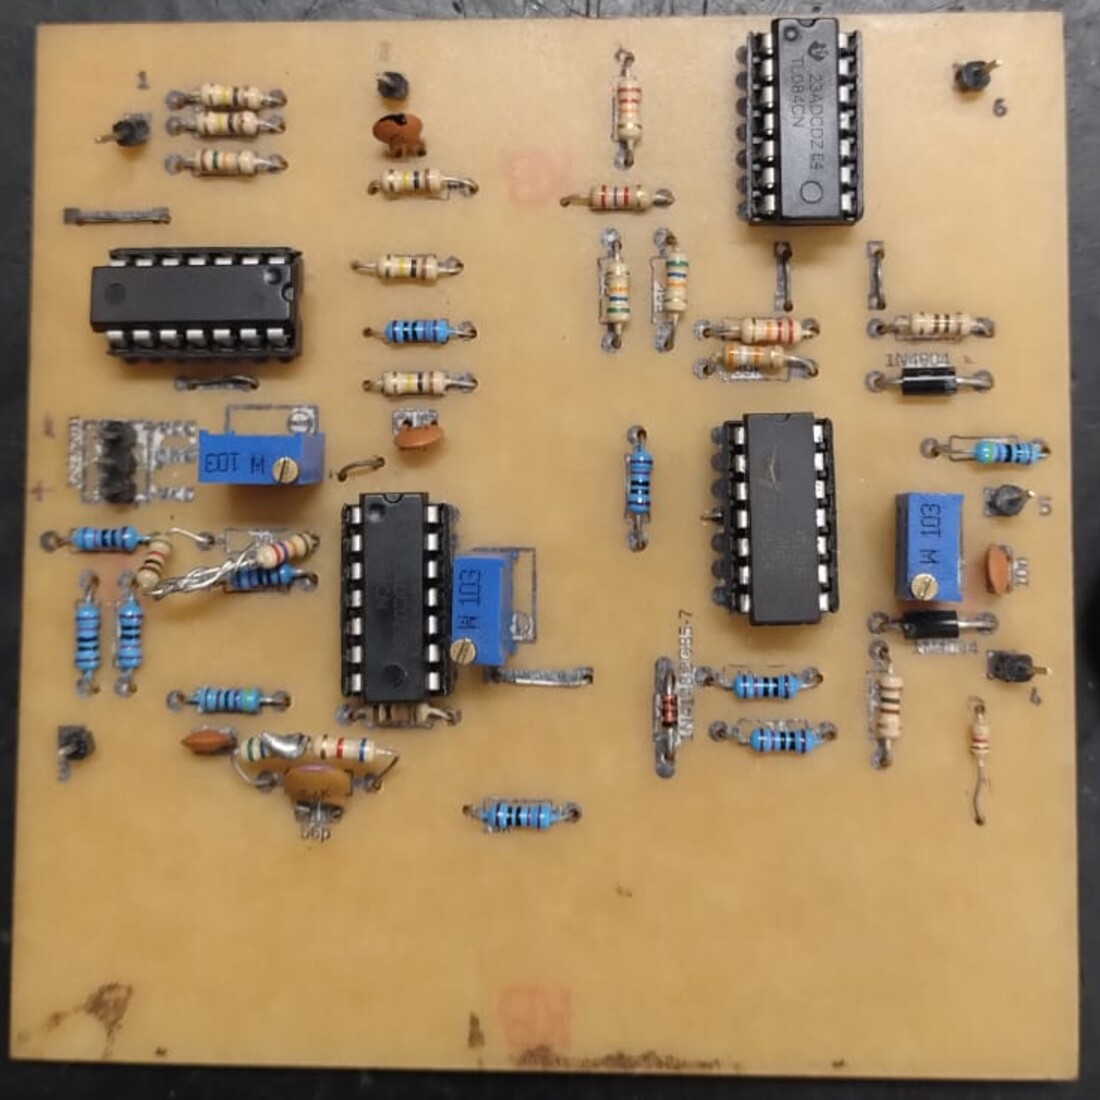
\includegraphics[width=\linewidth]{figuras/placa_superior.jpg}
\caption{Lado de componentes.}
\end{subfigure}\hspace{0.04\textwidth}%
\begin{subfigure}[b]{0.42\textwidth}
\centering
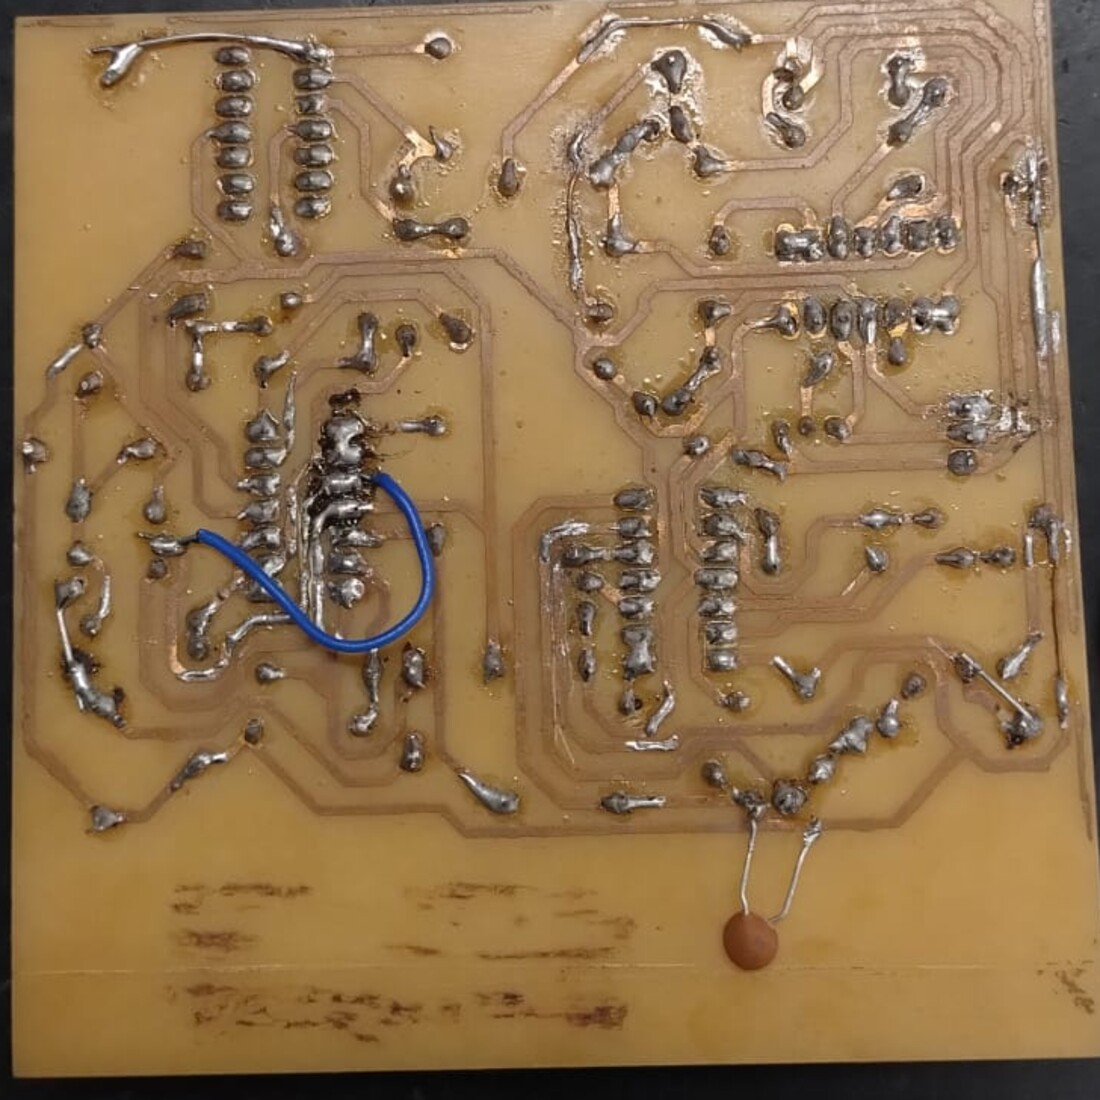
\includegraphics[width=\linewidth]{figuras/placa_inferior.jpg}
\caption{Lado de pistas.}
\end{subfigure}
\caption{Placa ensayada.}
\label{fig:placa}
\end{figure*}

\begin{table}[!htb]
\centering
\caption{Lista de componentes.}
\label{tab:bom}
\footnotesize
\setlength{\tabcolsep}{3pt}
\begin{tabular}{@{}>{\raggedright}p{2.5cm}l>{\raggedright\arraybackslash}p{3.2cm}@{}}
\toprule
\textbf{Referencia} & \textbf{Valor} & \textbf{Tipo} \\
\midrule
U1, U2, U3 & TL084CN & DIP-14 \\
$R_1$, $R_9$ & \SI{15}{\kilo\ohm} & Película metálica, \SI{1}{\percent} \\
$R_2$ a $R_8$, $R_{10}$ a $R_{13}$, $R_{15}$, $R_{F8}$ & \SI{10}{\kilo\ohm} & Película metálica, \SI{1}{\percent} \\
$R_{14}$ & \SI{20}{\kilo\ohm} & Película metálica, \SI{1}{\percent} \\
$R_I$ & \SI{5,6}{\kilo\ohm} & Película metálica, \SI{1}{\percent} \\
$R_F$ & \SI{1}{\mega\ohm} & Película metálica, \SI{1}{\percent} \\
$R_D$ & \SI{31,6}{\kilo\ohm} & Película metálica, \SI{1}{\percent} (E96) \\
$R_S$ & \SI{1}{\kilo\ohm} & Película metálica, \SI{1}{\percent} \\
$R_{S4}$, $R_{F4}$ & \SI{4,7}{\kilo\ohm} & Película metálica, \SI{1}{\percent} \\
$R_Z$ & \SI{470}{\ohm} & Película metálica, \SI{0,25}{\watt} \\
$P_1$, $P_2$, $P_3$ & \SI{10}{\kilo\ohm} & Preset multivuelta \\
$C_1$ & \SI{4,7}{\nano\farad} & Poliéster, \SI{5}{\percent} \\
$C_D$, $C_4$ & \SI{1}{\nano\farad} & Poliéster, \SI{5}{\percent} \\
$C_F$ & \SI{56}{\pico\farad} & Cerámico NP0 \\
$C_C$ & \SI{1}{\micro\farad} & Poliéster \\
Desacople (por integrado) & \SI{100}{\nano\farad} + \SI{10}{\micro\farad} & Cerámico + electrolítico \\
$D_{Z1}$ & 1N750 & Zener \SI{4,7}{\volt}, \SI{500}{\milli\watt} \\
$D_1$, $D_2$ & 1N4004 & Rectificador \SI{1}{\ampere} \\
\bottomrule
\end{tabular}
\end{table}

\subsection{Procedimiento de ajuste}
\label{sec:ajuste}
Los tres presets se ajustan en el orden en que afectan a las señales, porque cada uno cambia todo lo que está después:
\begin{enumerate}[leftmargin=*, nosep]
    \item Sin señal de entrada, verificar las tensiones de alimentación y la del zener.
    \item Con un multímetro en la salida de U1B, llevar $\Vrefd$ a \SI{1,25}{\volt} con $P_1$; con el multímetro en la salida de U2D, llevar $\Vrefu$ a \SI{1}{\volt} con $P_2$.
    \item Conectar el generador (cuadrada de \SI{0}{} a \SI{2,5}{\volt}, \SI{4,3}{\kilo\hertz}) y esperar un segundo, para que se cargue $C_C$.
    \item Con el osciloscopio en continua, verificar que la señal 1 vaya de \SI{-1}{} a \SI{1,5}{\volt}; si no, retocar $P_2$. Medir el valor medio de la señal 2 con el multímetro y, si no es \SI{1,25}{\volt}, retocar $P_1$: así se compensan también los \emph{offsets} de los operacionales.
    \item Ajustar $P_3$ para que los impulsos de la señal 4 tengan \SI{1}{\volt} de pico.
\end{enumerate}

\subsection{Medición}
La placa se alimentó con la fuente partida del laboratorio y se excitó con el generador de funciones ajustado a una cuadrada de \SI{0}{} a \SI{2,5}{\volt} y \SI{4,3}{\kilo\hertz}. Las señales se registraron con un osciloscopio digital Rigol, en continua; la Fig.~\ref{fig:capturas} reúne las seis capturas.

Para compararlas con la simulación se digitalizaron. Cada captura tiene una retícula de 12 por 8 divisiones de 25 píxeles, así que cada píxel equivale a $1/25$ de división en tensión y en tiempo, y la traza amarilla se convierte en una tabla tensión--tiempo. Con las bases de tiempo usadas, un píxel equivale a \SI{2}{\micro\second} en las capturas 1 a 3 y a \SI{4}{\micro\second} en las capturas 4 a 6, de modo que los detalles más breves que eso no se resuelven.

\begin{figure*}[!t]
\centering
\begin{subfigure}[b]{0.32\textwidth}
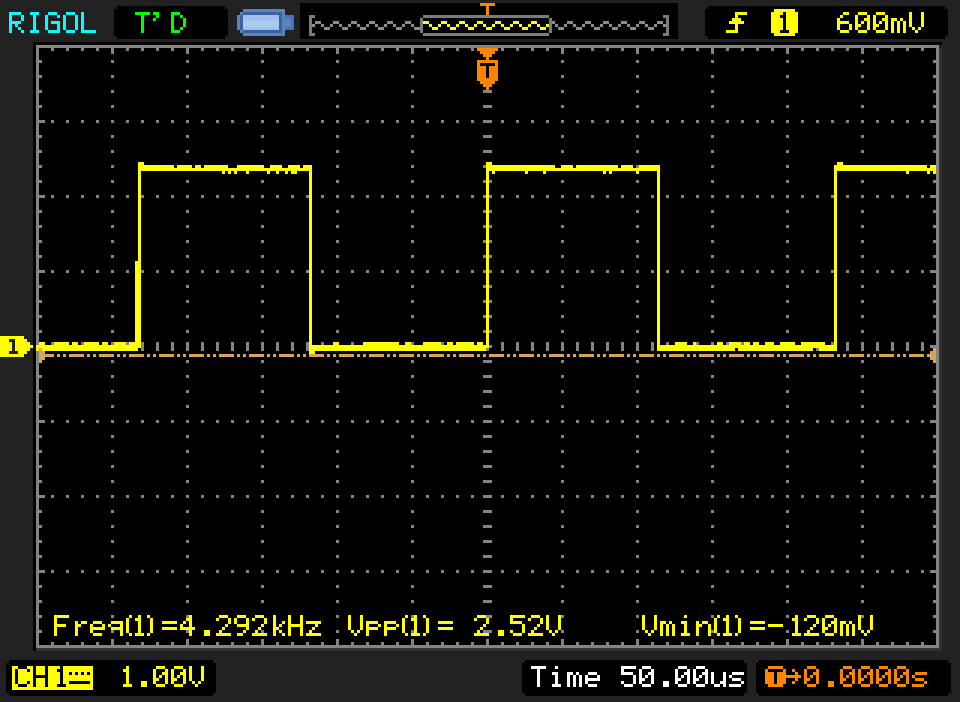
\includegraphics[width=\linewidth]{figuras/osc_1.png}
\caption{Entrada (\SI{1}{\volt\per div}, \SI{50}{\micro\second\per div}).}
\end{subfigure}\hfill
\begin{subfigure}[b]{0.32\textwidth}
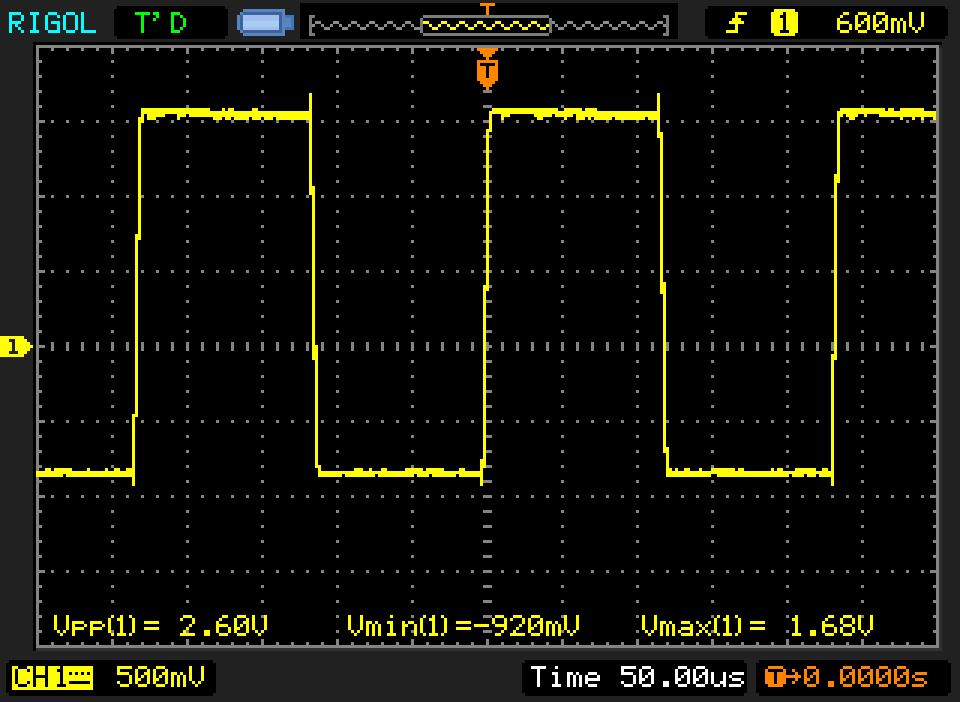
\includegraphics[width=\linewidth]{figuras/osc_2.png}
\caption{Señal 1 (\SI{0,5}{\volt\per div}, \SI{50}{\micro\second\per div}).}
\end{subfigure}\hfill
\begin{subfigure}[b]{0.32\textwidth}
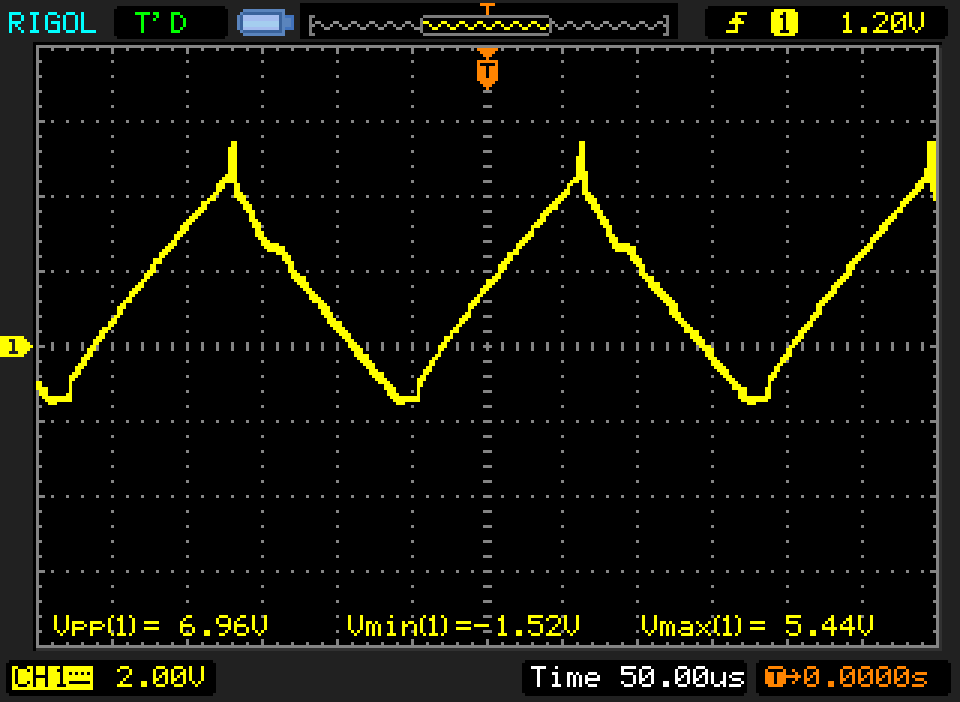
\includegraphics[width=\linewidth]{figuras/osc_3.png}
\caption{Señal 2 (\SI{2}{\volt\per div}, \SI{50}{\micro\second\per div}).}
\end{subfigure}\\[4pt]
\begin{subfigure}[b]{0.32\textwidth}
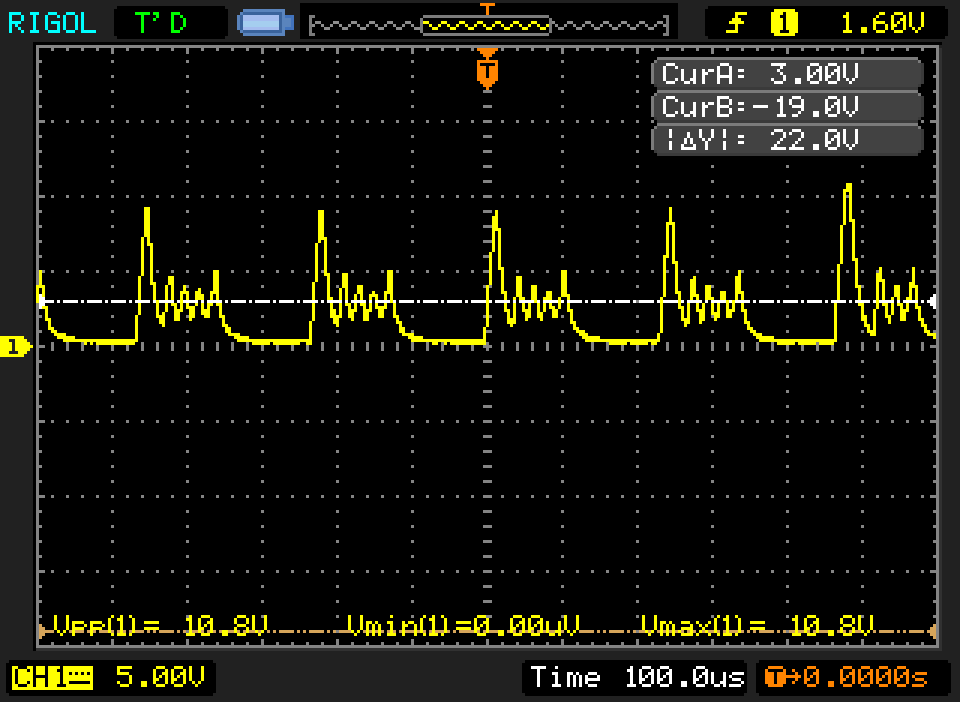
\includegraphics[width=\linewidth]{figuras/osc_4.png}
\caption{Señal 4 (\SI{5}{\volt\per div}, \SI{100}{\micro\second\per div}).}
\end{subfigure}\hfill
\begin{subfigure}[b]{0.32\textwidth}
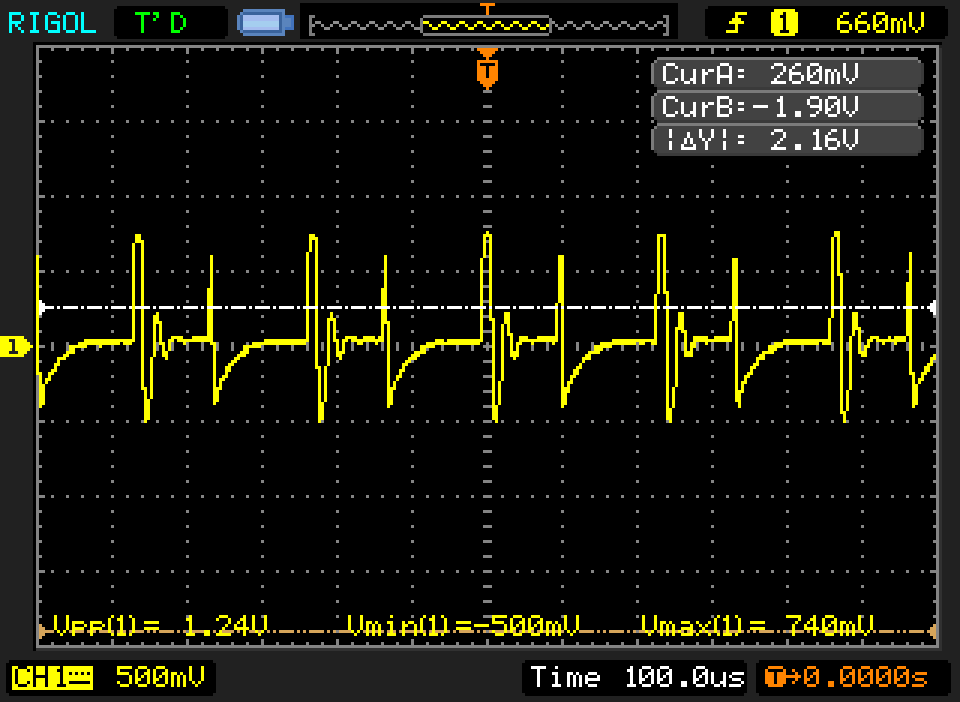
\includegraphics[width=\linewidth]{figuras/osc_5.png}
\caption{Impulsos $v_p$ (\SI{0,5}{\volt\per div}, \SI{100}{\micro\second\per div}).}
\end{subfigure}\hfill
\begin{subfigure}[b]{0.32\textwidth}
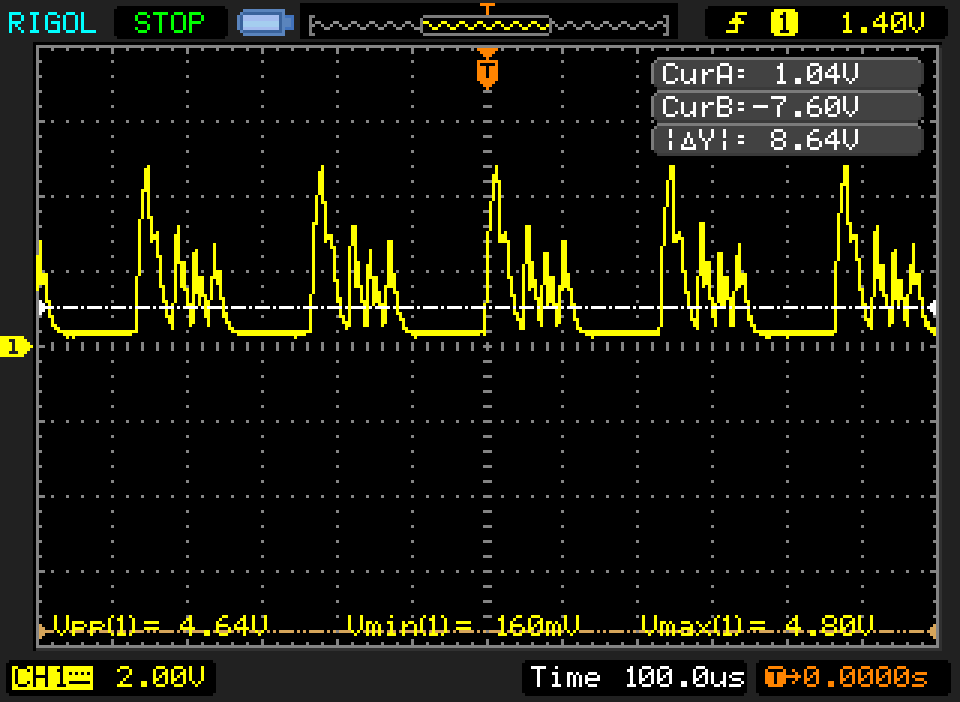
\includegraphics[width=\linewidth]{figuras/osc_6.png}
\caption{Señal 4 (\SI{2}{\volt\per div}, \SI{100}{\micro\second\per div}).}
\end{subfigure}
\caption{Capturas del osciloscopio. El marcador ``1'' del borde izquierdo indica el cero del canal en todas las capturas.}
\label{fig:capturas}
\end{figure*}

\subsection{Resultados: entrada, señal 1 y señal 2}
\label{sec:resultados}
La entrada (captura 1) es una cuadrada de \valu{2}{\medInBajo}{\volt} a \valu{2}{\medInAlto}{\volt} y \valu{3}{\medFrec/1000}{\kilo\hertz} según la medición automática del osciloscopio, con el nivel alto durante un \valu{0}{\medCiclo}{\percent} del período. La amplitud es un \valu{0}{100*(2.5-(\medInAlto-\medInBajo))/2.5}{\percent} menor que la nominal y la frecuencia, un \valu{1}{100*(4300-\medFrec)/4300}{\percent} menor.

La señal 1 (captura 2) tiene mesetas en \valu{2}{\medSUnoBajo}{\volt} y \valu{2}{\medSUnoAlto}{\volt}. Su excursión, \valu{2}{\medSUnoAlto-\medSUnoBajo}{\volt}, es la de la entrada: la ganancia del restador es 1, como se diseñó. La señal 2 (captura 3) es una triangular con rampas rectas, que sube mientras la señal 1 está en alto. Para no confundir sus vértices con los picos que aparecen sobre ellos, se calcularon intersecando rectas ajustadas a las rampas: \valu{2}{\medSDosVertMin}{\volt} y \valu{2}{\medSDosVertMax}{\volt}, con pendientes de \valu{1}{1000*\medSDosPendSub}{\volt\per\milli\second} y \valu{1}{1000*\medSDosPendBaj}{\volt\per\milli\second}.

Para comparar con la simulación sin mezclar los errores de ajuste con los de diseño, se repitió la simulación del circuito completo con la entrada medida (\valu{2}{\medInBajo}{\volt} a \valu{2}{\medInAlto}{\volt}, \valu{0}{\medFrec}{\hertz}) y con $P_2$ en la posición que reproduce el nivel medido de la señal 1. La Fig.~\ref{fig:medsim} superpone el resultado con las capturas 2 y 3, y la Tabla~\ref{tab:medicion} resume la comparación. La señal 1 simulada coincide con la medida en las dos mesetas, y la triangular medida tiene la forma, la fase y la linealidad de la simulada. Sus diferencias de amplitud y de nivel se analizan en la Sección~\ref{sec:problemas}.

\begin{figure}[!htb]
\centering
\begin{tikzpicture}
\begin{groupplot}[
    group style={group size=1 by 2, vertical sep=6pt, xticklabels at=edge bottom},
    tp2, height=3.8cm, xmin=0, xmax=600, xtick={0,100,...,600},
]
\nextgroupplot[ylabel={S1 [V]}, ymin=-1.4, ymax=2.5, ytick={-1,0,1,2}, legend pos=north east, legend columns=2]
\addplot[cmed, line width=1.6pt] table[x=t, y=v] {datos/med2.dat};
\addplot[cs1] table[x=t, y=s1] {datos/medida_sim.dat};
\legend{Medida, Simulada}
\nextgroupplot[ylabel={S2 [V]}, ymin=-2.4, ymax=6.4, ytick={-2,0,2,4,6}, xlabel={Tiempo [\si{\micro\second}]}]
\addplot[cmed, line width=1.6pt] table[x=t, y=v] {datos/med3.dat};
\addplot[cs2] table[x=t, y=s2] {datos/medida_sim.dat};
\end{groupplot}
\end{tikzpicture}
\caption{Capturas 2 y 3 digitalizadas, superpuestas con la simulación del circuito excitado con la entrada medida y con $P_2$ en la posición del ensayo.}
\label{fig:medsim}
\end{figure}

\begin{table}[!htb]
\centering
\caption{Comparación entre la medición y la simulación con la entrada medida.}
\label{tab:medicion}
\footnotesize
\setlength{\tabcolsep}{3pt}
\begin{tabular}{@{}llccc@{}}
\toprule
\textbf{Señal} & \textbf{Magnitud} & \textbf{Consigna} & \textbf{Simulada} & \textbf{Medida} \\
\midrule
Entrada & Bajo / alto [\si{\volt}] & 0 / 2,5 & \multicolumn{2}{c}{\val{2}{\medInBajo} / \val{2}{\medInAlto}} \\
 & Frecuencia [\si{\hertz}] & 4300 & \multicolumn{2}{c}{\val{0}{\medFrec}} \\
\midrule
S1 & Bajo / alto [\si{\volt}] & $-1$ / 1,5 & \val{2}{\simMedSunoBajo} / \val{2}{\simMedSunoAlto} & \val{2}{\medSUnoBajo} / \val{2}{\medSUnoAlto} \\
\midrule
\multirow{4}{*}{S2} & Mín. / máx. [\si{\volt}] & $-1{,}5$ / 4 & \val{2}{\simMedSdosMin} / \val{2}{\simMedSdosMax} & \val{2}{\medSDosVertMin} / \val{2}{\medSDosVertMax} \\
 & Pico a pico [\si{\volt}] & 5,5 & \val{2}{\simMedSdosVpp} & \val{2}{\medSDosVertVpp} \\
 & Nivel medio [\si{\volt}] & 1,25 & \val{2}{\simMedSdosMed} & \val{2}{\medSDosVertCentro} \\
 & Pend. sub. / baj. [\si{\volt\per\milli\second}] & $\pm 47{,}3$ & $\pm$\val{1}{(\simMedSdosVpp)/(0.5e3/\medFrec)} & \val{1}{1000*\medSDosPendSub} / \val{1}{1000*\medSDosPendBaj} \\
\midrule
\multirow{2}{*}{S4} & Impulsos por período & 2 & 2 & 1 \\
 & Pico [\si{\volt}] & 1 & 1,00 & \val{1}{\medCSeisMax} y \val{1}{\medCCuatroMax} \\
\bottomrule
\end{tabular}
\end{table}

\section{Problemas encontrados}
\label{sec:problemas}
Las dos primeras etapas funcionaron como se diseñaron, pero la medición tuvo errores de procedimiento y la señal 4 no salió como la simulada. Esta sección analiza cada problema, en el orden de la cadena de señales, y usa la simulación para separar lo que se explica por el ajuste o por la medición de lo que indica una falla de la etapa.

\subsection{Presets sin ajustar antes de medir}
Las capturas muestran que los presets no estaban en su posición de diseño cuando se registraron las señales:
\begin{itemize}[leftmargin=*, nosep]
    \item La señal 1 está \valu{2}{\medSUnoBajo+1}{\volt} por encima de lo pedido: la etapa restó \valu{2}{\simAjVrefUno}{\volt} en vez de \SI{1}{\volt}, es decir, $P_2$ daba $\Vrefu = \valu{2}{\simAjVrefUno}{\volt}$. Con ese valor, la simulación reproduce las dos mesetas medidas (Tabla~\ref{tab:medicion}).
    \item El nivel medio de la triangular está \valu{2}{\medSDosVertCentro-1.25}{\volt} por encima de \SI{1,25}{\volt}. Con el integrador acoplado en alterna, ese nivel es $\Vrefd$ más los \emph{offsets} de U1D y U2A, que no superan \SI{60}{\milli\volt}; la diferencia restante corresponde a la posición de $P_1$.
\end{itemize}
El error fue capturar las señales sin completar los pasos 2 y 4 del procedimiento de la Sección~\ref{sec:ajuste}. Ninguno de los dos desvíos indica un problema del circuito: los dos niveles están dentro del rango de sus presets.

\subsection{Amplitud y asimetría de la triangular}
La triangular medida tiene \valu{2}{\medSDosVertVpp}{\volt} pico a pico, un \valu{0}{100*(\medSDosVertVpp/\simMedSdosVpp-1)}{\percent} más que la simulada con la misma entrada. Como la amplitud es proporcional a $1/(R_I C_1)$, equivale a una constante de tiempo un \valu{0}{100*(1-\simMedSdosVpp/\medSDosVertVpp)}{\percent} menor que la nominal. Eso es más de lo que cubre la simulación con tolerancias del \SI{5}{\percent} (Tabla~\ref{tab:mc}), así que el capacitor de integración se aparta de su valor nominal más de lo supuesto. Debió medirse $C_1$ antes de montarlo; el diseño no tiene un ajuste para esta amplitud, y una mejora sería poner un preset en serie con $R_I$.

Además, la pendiente de subida es un \valu{0}{100*(\medSDosPendSub/(-\medSDosPendBaj)-1)}{\percent} mayor que la de bajada. Esto no es un defecto del circuito sino de la entrada: el generador tenía el nivel alto durante el \valu{0}{\medCiclo}{\percent} del período, así que el valor medio de la señal 1 quedó más cerca de su nivel bajo y la desviación respecto de ese valor medio, que es lo que integra el integrador, fue mayor en el semiperíodo alto. El ciclo de trabajo del generador debió verificarse y corregirse antes de medir.

\subsection{Picos en los vértices y quiebre de la rampa}
Sobre los vértices de la triangular hay picos de uno o dos píxeles de ancho (hasta \valu{1}{\medSDosMax}{\volt} en el superior), sincronizados con los flancos de la señal 1, que la simulación no tiene. Por su duración, de pocos microsegundos, y porque no dependen de la pendiente, se atribuyen al acoplamiento de los flancos de la señal 1 (\SI{2,5}{\volt} en \SI{0,2}{\micro\second}) a la punta del osciloscopio, a través del cable de masa largo de la punta o de capacidades parásitas. No hay capturas tomadas con el resorte de masa corto de la punta, que es la prueba que permitiría confirmarlo.

En la rampa de bajada, unos \SI{30}{\micro\second} después del máximo, la pendiente se reduce durante unos \SI{15}{\micro\second}. Este quiebre importa porque la etapa siguiente es un derivador: cualquier cambio de pendiente de la señal 2 se convierte en un escalón de la señal 3 y, por lo tanto, en un impulso de más en la señal 4. Con una sola captura y un solo canal no se pudo establecer si el quiebre está en la señal o es otra vez un efecto de la medición.

\subsection{Limitaciones de la medición}
Antes de analizar la señal 4 conviene marcar lo que la medición no permite saber:
\begin{itemize}[leftmargin=*, nosep]
    \item \textbf{Un solo canal.} Cada captura tiene una sola señal, así que no hay referencia de fase entre etapas: no se puede verificar en la placa que la señal 3 cambie en los vértices de la triangular.
    \item \textbf{Falta la señal 3.} No se guardó ninguna captura de la señal 3, que es justamente la entrada de la etapa que falla.
    \item \textbf{Base de tiempo demasiado lenta.} La señal 4 se registró a \SI{100}{\micro\second\per div}, donde cada píxel abarca \SI{4}{\micro\second}. Una oscilación del orden de \SI{100}{\kilo\hertz}, como la que tendría un derivador mal amortiguado (Sección~\ref{sec:derivador}), no se puede representar con esa resolución: la captura muestra que hay oscilación y cuánto dura, pero no su frecuencia.
    \item \textbf{Condiciones no registradas.} Las capturas 4 y 6 muestran la misma forma con amplitudes muy distintas, y no quedó anotado qué cambió entre una y otra.
\end{itemize}

\subsection{Señal 4: síntomas}
En las capturas 4 a 6 la etapa de impulsos se aparta del diseño en tres aspectos:
\begin{itemize}[leftmargin=*, nosep]
    \item \textbf{Un impulso dominante por período}. Hay un solo impulso grande cada \valu{0}{\medCSeisPeriodo}{\micro\second}, es decir, uno por período, de \valu{1}{\medCSeisMax}{\volt} en la captura 6 y \valu{1}{\medCCuatroMax}{\volt} en la 4. El diseño da dos impulsos iguales por período, de \SI{1}{\volt}.
    \item \textbf{Ráfagas de oscilación}. Después de cada impulso dominante aparecen varios picos menores durante unos \SI{100}{\micro\second}, con una separación aparente de unos \valu{0}{\medCSeisRafaga}{\micro\second}, que por lo dicho no es su período real.
    \item \textbf{Eventos no equidistantes}. En $v_p$ (captura 5) hay dos eventos por período, pero separados alternadamente unos \valu{0}{\medCCincoSep}{\micro\second} y \valu{0}{\medCCincoPeriodo-\medCCincoSep}{\micro\second}, en vez de \SI{116}{\micro\second}, y sus amplitudes, \valu{2}{\medCCincoMax}{\volt} y \valu{2}{\medCCincoMin}{\volt}, son menores que los $\pm\SI{1,6}{\volt}$ del diseño.
\end{itemize}

\subsection{Señal 4: causas posibles}
\label{sec:fallas}
Como las capturas no alcanzan para ubicar la causa, se simuló el circuito completo con defectos introducidos a propósito, de los que pueden ocurrir en esta etapa por un componente equivocado o mal soldado. Dos de ellos reproducen los síntomas principales:
\begin{itemize}[leftmargin=*, nosep]
    \item \textbf{Derivador poco amortiguado}: $R_S = \SI{330}{\ohm}$ y sin $C_F$. La señal 3 oscila después de cada vértice y el generador de impulsos, que es un pasaaltos, deja pasar esa oscilación. En la salida aparecen ráfagas después de cada impulso, con picos de hasta \valu{1}{\simFallaAmortMax}{\volt}.
    \item \textbf{Sumador desbalanceado}: $R_{14} = R_{15}$ en lugar de $R_{14} = 2R_{15}$. Como se vio en la Sección~\ref{sec:s4}, los impulsos positivos de $v_p$ se cancelan y los negativos salen con el doble de amplitud: un solo impulso por período, de \valu{1}{\simFallaSumadorPicoSub}{\volt}, y \valu{2}{\simFallaSumadorPicoBaj}{\volt} en el otro flanco.
\end{itemize}
Con los dos defectos a la vez, la salida simulada tiene un impulso dominante de \valu{1}{\simFallaAmbasPicoSub}{\volt} por período seguido de una ráfaga, como la captura 6. La Fig.~\ref{fig:fallas} superpone ambas.

\begin{figure}[!htb]
\centering
\begin{tikzpicture}
\begin{axis}[tp2, height=4.8cm, xmin=0, xmax=1200, ymin=-1.2, ymax=5.8,
    xlabel={Tiempo [\si{\micro\second}]}, ylabel={S4 [V]}, legend pos=north west, legend columns=2]
\addplot[cmed, line width=1.5pt] table[x=t, y=v] {datos/med6.dat};
\addplot[cs4, line width=0.5pt] table[x expr=\thisrow{t}+\simFallaDesfase, y=s4ambas] {datos/fallas.dat};
\legend{Captura 6, Simulación con ambos defectos}
\end{axis}
\end{tikzpicture}
\caption{Señal 4 medida (captura 6 digitalizada) y simulada con el derivador poco amortiguado y el sumador desbalanceado.}
\label{fig:fallas}
\end{figure}

La coincidencia no es completa, y conviene marcar sus límites. La simulación no explica la amplitud de la captura 4 (\valu{1}{\medCCuatroMax}{\volt}), que ni con la ganancia máxima de $P_3$ se alcanza; como tiene la misma forma y el mismo período que la captura 6, lo más probable es que entre ambas haya cambiado el estado de la oscilación o un ajuste, que no quedó registrado. Tampoco explica la separación desigual de los eventos de la captura 5, porque en el circuito simulado los flancos de la señal 3 coinciden siempre con los vértices de la triangular; el quiebre de la rampa de bajada de la triangular es una explicación posible.

Lo que sí establece la simulación es que el diseño nominal no produce ninguno de estos síntomas: con la compensación de la Sección~\ref{sec:derivador} el derivador no oscila, y con la relación 2:1 el rectificador da impulsos iguales en ambos flancos (Fig.~\ref{fig:nominal}). Para completar el ensayo de esta etapa habría que:
\begin{enumerate}[leftmargin=*, nosep]
    \item medir la señal 3 con una base de tiempo de \SI{5}{\micro\second\per div} o menos alrededor de un vértice, para confirmar la oscilación, y verificar $R_S$ y $C_F$;
    \item medir $R_{14}$ y $R_{15}$ fuera del circuito y confirmar la relación 2:1;
    \item observar la señal 1 y la señal 2 a la vez con los dos canales, con el resorte de masa corto de la punta, para ubicar el quiebre de la rampa respecto de los flancos de la entrada;
    \item reemplazar los 1N4004 por 1N4148 (Sección~\ref{sec:s4}) y volver a ajustar $P_3$.
\end{enumerate}

\section{Conclusiones}
\label{sec:conclusiones}

\paragraph*{Diseño} El circuito obtiene las cuatro señales de la consigna en el orden pedido y cada una a partir de la anterior, con tres TL084 y $\pm\SI{12}{\volt}$. El TL084 se eligió por su entrada JFET, que hace despreciable el error por corriente de polarización en el integrador, por su \emph{slew rate}, que el rectificador necesita para conmutar dentro de impulsos de pocos microsegundos, y porque tiene cuatro amplificadores por integrado. La impedancia de entrada es de \SI{15}{\kilo\ohm}, fijada por un resistor y un seguidor, y la de salida es de \valu{2}{\simZoutF}{\ohm} a la frecuencia de trabajo; como es inductiva ($L_{eq} \approx \valu{0}{\teoLeq}{\micro\henry}$), se mide inyectando corriente y no con el método de la carga.

\paragraph*{Niveles de continua} Los niveles salen de un zener con presets y seguidores, y no de divisores sobre la fuente, y ninguna etapa amplifica la continua con ganancia mayor que 2: cada amplitud se fija en la etapa que genera la señal. El punto crítico fue el integrador. Con una resistencia en paralelo hay que elegir entre rampas rectas y un nivel estable: con $R_F/R_I = 100$, \SI{50}{\milli\volt} de error en la entrada mueven la triangular \valu{1}{\simIntDcCienCorr}{\volt}. El capacitor en serie con $R_I$ resuelve ese compromiso: la triangular queda centrada en la referencia de \SI{1,25}{\volt}, como pide la consigna, con una alinealidad del \valu{2}{\simIntAcNoLin}{\percent}.

\paragraph*{Estabilidad y velocidad} La señal 3 se obtuvo con un derivador y no con un comparador, porque un comparador contra el nivel medio la habría atrasado un cuarto de período. Sin compensar, ese derivador oscila a unos \SI{130}{\kilo\hertz}; con $R_S = \SI{1}{\kilo\ohm}$ y $C_F = \SI{56}{\pico\farad}$ el sobrepico baja al \valu{1}{\simBarrDSobrepico}{\percent}, al costo de flancos de unos \SI{4}{\micro\second}. El rectificador de precisión funciona con 1N4004, aunque con 1N4148 el pulso negativo de conmutación sería la mitad.

\paragraph*{Implementación} En la placa, la señal 1 coincidió con la simulación hecha con la entrada medida, y la triangular tuvo la forma, la fase y la linealidad del diseño.

\paragraph*{Lo que salió mal} Los niveles de las señales 1 y 2 quedaron corridos porque se midió sin terminar de ajustar los presets, y la triangular salió un \valu{0}{100*(\medSDosVertVpp/\simMedSdosVpp-1)}{\percent} más grande porque el capacitor de integración se apartaba de su valor nominal. La señal 4 tuvo un solo impulso dominante por período y ráfagas de oscilación. Las capturas no alcanzaron para ubicar la causa: hay un solo canal por captura, no se registró la señal 3 y la base de tiempo no resolvía la oscilación. La simulación muestra que el diseño nominal no produce esos síntomas y que los reproducen un derivador poco amortiguado y un desbalance en la red sumadora del rectificador; las mediciones para confirmarlo están al final de la Sección~\ref{sec:fallas}.

\paragraph*{Aprendizajes} La simulación con el macromodelo del fabricante fue indispensable en las dos etapas que dependen de la dinámica del operacional, el derivador y el rectificador: con un operacional ideal ninguna de las dos muestra problemas. También lo fue para interpretar las mediciones, porque comparando las capturas con el circuito simulado, con y sin defectos, se pudo descartar un error de diseño y acotar dónde buscar. De la medición queda una lección práctica: ajustar los presets antes de capturar, medir con dos canales para tener referencia de fase y elegir la base de tiempo según el detalle que se quiere ver, no según el período de la señal.


\begin{thebibliography}{99}
\bibitem{linares-intro}
F. Linares, \emph{Amplificadores operacionales: introducción}. Práctico de Electrónica Aplicada II, UTN FRC, versión 2020.

\bibitem{linares-intder}
F. Linares, \emph{Amplificadores operacionales: integradores y derivadores}, rev.~02. Práctico de Electrónica Aplicada II, UTN FRC.

\bibitem{linares-comp}
F. Linares, \emph{A.O.: comparadores, multiplicadores, convertidores}. Práctico de Electrónica Aplicada II, UTN FRC, versión 2020.

\bibitem{refs}
P. Miller y D. Moore, ``Precision voltage references'', \emph{Analog Applications Journal}, Texas Instruments, nov. 1999.

\bibitem{tl08x}
Texas Instruments, \emph{TL08xx JFET-input operational amplifiers}, hoja de datos SLOS081I, rev. may. 2015.

\bibitem{opamps}
Texas Instruments, \emph{LM741 operational amplifier} y \emph{LMx24 quadruple operational amplifiers}; Analog Devices, \emph{OP07 ultralow offset voltage operational amplifier}. Hojas de datos.

\bibitem{1n750}
onsemi, \emph{1N746A--1N759A, 500 mW DO-35 hermetically sealed glass zener voltage regulators}, hoja de datos.

\bibitem{1n4004}
Vishay General Semiconductor, \emph{1N4001 thru 1N4007: general purpose plastic rectifier}, hoja de datos 88503.

\bibitem{1n4148}
onsemi, \emph{1N914, 1N4148: high conductance fast diode}, hoja de datos.

\bibitem{coughlin}
R. F. Coughlin y F. F. Driscoll, \emph{Amplificadores operacionales y circuitos integrados lineales}, 5.ª ed. México: Prentice Hall, 1999.

\bibitem{franco}
S. Franco, \emph{Design with Operational Amplifiers and Analog Integrated Circuits}, 4.ª ed. Nueva York: McGraw-Hill, 2015.

\bibitem{ngspice}
H. Vogt, G. Atkinson y P. Nenzi, \emph{Ngspice User's Manual}, versión 47. [En línea]. Disponible: \url{https://ngspice.sourceforge.io}
\end{thebibliography}

\end{document}
